\documentclass{article}
\usepackage{graphicx}
\begin{document}
	
	\section*{Notizen Lineare Algebra}
	\subsection*{Roadmap zur LA Klausur}
	1. Lineare Gleichungssysteme (auch Ungleichungen) \\
	Lineare Optimierung \\
	2. Analytische Geometrie: Vektorrechnung!!! \\
	Vektoren, Addieren Betrag etc. \\
	3. Matrizen \\
	Produktionsprozesse, Übergansmatrizen 
	4. Lineare Abbildungen \\
	Abbildungsmatrix, Umrechnung der Basis \\
	5. Eigenwerte Eigenvektoren \\
	Eigenwerte und -vektoren bestimmen, Diagonalisierbarkeit \\
	6. Algebraische Strukturen \\
	Körper, komplexe Zahlen: Formenwechsel und Gleichungen
	
	\subsection*{13.04.2021}
	
	Lineare (Un-)Gleichungssysteme \\
	Analytische Geometrie  \\
	Matrizen \\
	Lineare Abbildungen  \\
	Algebraische Strukturen \\
	\\
	für LGS müssen Gleichungen linear sein. \\
	1. Grades \\
	m x n (m kreuz n) besteht aus m Zeilen und n Spalten. \\
	LGS ist homogen wenn rechte Seite immer = 0. \\
	Ansonsten inhomogen \\
	Homogene LGS haben immer eine Lösung. \\
	Anwendung CT \\
	Gauß Algorithmus Kap 1 Folie 20 \\
	Dreiecksform herstellen \\
	Gleichungen von unten nach oben lösen. \\
	LGS hat eine, keine oder unendlich viele Lösungen. \\
	\subsection*{20.04.2021}
	Gauß-Algorithmus braucht viele Multiplikationen \\
	$\sum_{k=1}^{n-1}$k * (k+2) =  \\
	Der Gauß-Algorithmus erfordert $(n^3 + 3n^2 -n)*1/3$ Multiplikationen. \\
	Gauß-Algorithmus braucht ca 2 Wochen für CT. \\
	Mit Iteration um den Faktor 45000 schneller. \\
	Lineare Optimierung \\
	Maximierung unter linearen Randbedingungen \\
	Es ergibt sich zu lösendes Ungleichungssystem. \\
	Zulässigkeitsbereich: Bereich der alle gültigen Lösungen enthält. \\
	Randbedingungen und Zielfunktion aufstellen. \\
	Ergebnis in der Regel ein Randpunkt des Zulässigkeitsbereich. \\
	Lösung Optimierungsproblem mit Halbenen und Zielfunktion als Gerade in Richtung des Optimums verschieben. \\
	Analytische Geometrie \\
	Untersuchen geometrischer Objekte. \\
	Vektoren, Punkte, Skalar- und Vektorprodukt \\
	Geraden, Ebene \\
	In 3D ablesen nicht mehr möglich.
	\subsection*{27.04.2021}
	Vektoren im Analytische Geometrie \\
	$
	\vec{e}_1= \left(\begin{array}{c} a \\ b \\ c \end{array}\right)
	$  \\
	Vektoren geben eine Verschiebung in eine  bestimmte Richtung mit genauer Länge an. \\
	Vektor zwischen zwei Punkten: Ziel - Start \\
	Ortsvektoren zeigen immer vom Ursprung zu einem Punkt P. \\
	Betrag eines Vektors mit Pythagoras Kap 2 F 16. \\
	Addition Kap 2 F 18 \\
	Gegenvektor \\
	Subtraktion ist definiert als Addition von a und dem Gegenvektor von b \\
	Rechengesetze von Vektorvervielfachung beachten kap 2 F 23 \\
	distributiv \\
	Linearkombination \\
	kolinear: Vektoren verlaufen parallel \\
	komplanar: Vektoren liegen in einer gemeinsamen Ebene \\
	lineare Abhängigkeit Kap 2 F 26. \\
	linearabhängige Vektoren können aus Linearkombinationen der anderen Vektoren dargestellt werden.\\
	Gerade g: Stützpunkt + Richtung * s \\
	Lage von zwei Geraden Kap 2 F 33 \\
	\section*{04.05.2021}
	Ebene E: $\vec{x} = s*\vec{u} + r*\vec{v}$ \\
	r und s werden gestreckt und gekürzt um jeden Punkt auf der Ebene als Linearkombination aus Stützvektor, u und v darzustellen. \\
	Koordinatengleichung \\
	Parametergleichung in Koordinatengleichung mit Gauß oder Normalvektor \\
	An K-Gleichung Achsenabschnitte ablesbar. \\
	Durchstoßpunkt: \\
	Gerade in Parameter einsetzen in K-Gleichung der Ebene. \\
	Dann Ergebnis dieser Gleichung als r in Gerade einsetzen. \\
	g und E echt parallel, wenn g in E = Widerspruch \\
	g in E wenn g in E allgemein gültig \\
	E und E parallel, identisch, Schnittgerade \\
	Verfahren ähnlich wie s.o. oder s. Kap 2 F 50 \\
	\subsection*{11.05.2021}
	Vektorprodukt Skalarprodukt \\
	def. Zweiu Vektoren a und b mit eingeschlossenen Winkel heißen $\phi$. \\
	$\vec{a}$ * $\vec{b}$ = $|$$\vec{a}$$|$ * $|$$\vec{a}$$|$ * $\cos$($\phi$) \\
	Sample Skalarprodukt in der Praxis: \\
	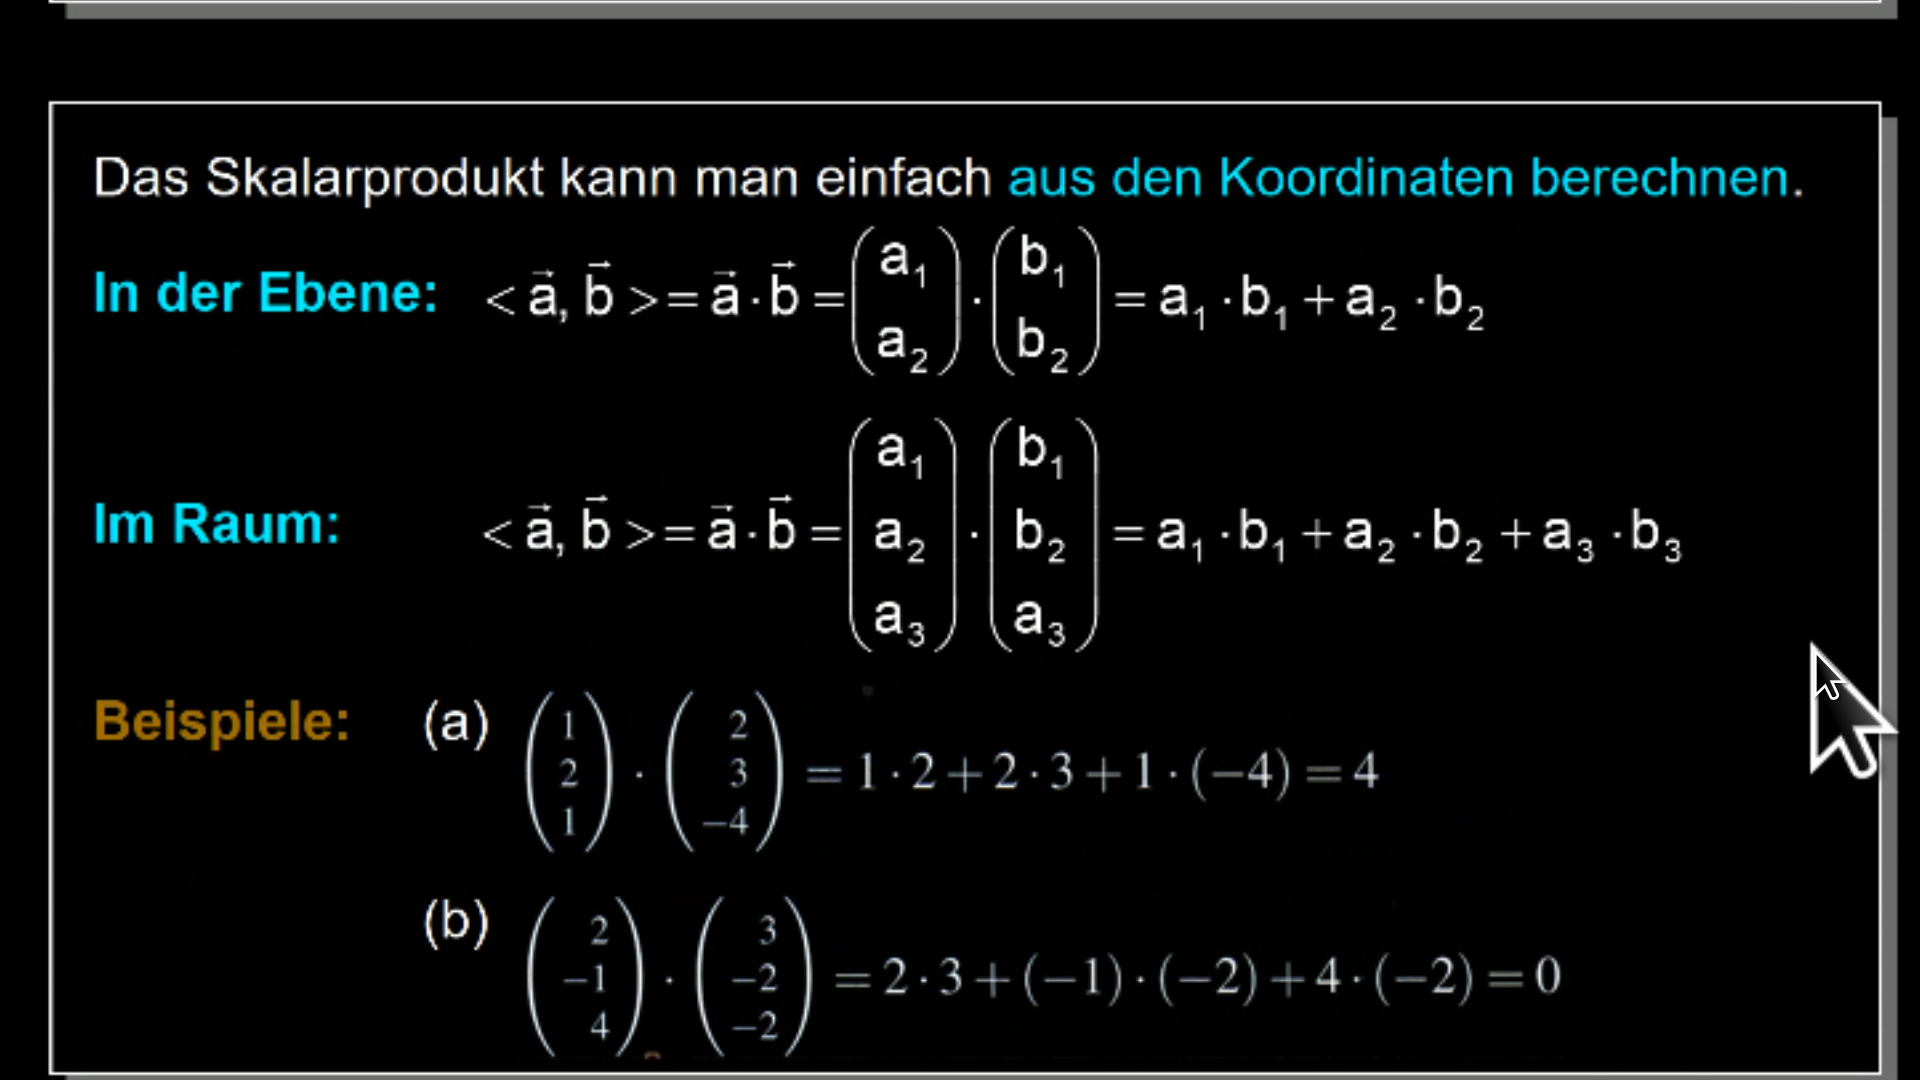
\includegraphics[width=\linewidth]{Pic01}
	\\
	Skalarprodukt ist kommutativ und distributiv aber nur eingeschränkt assoziativ. \\
	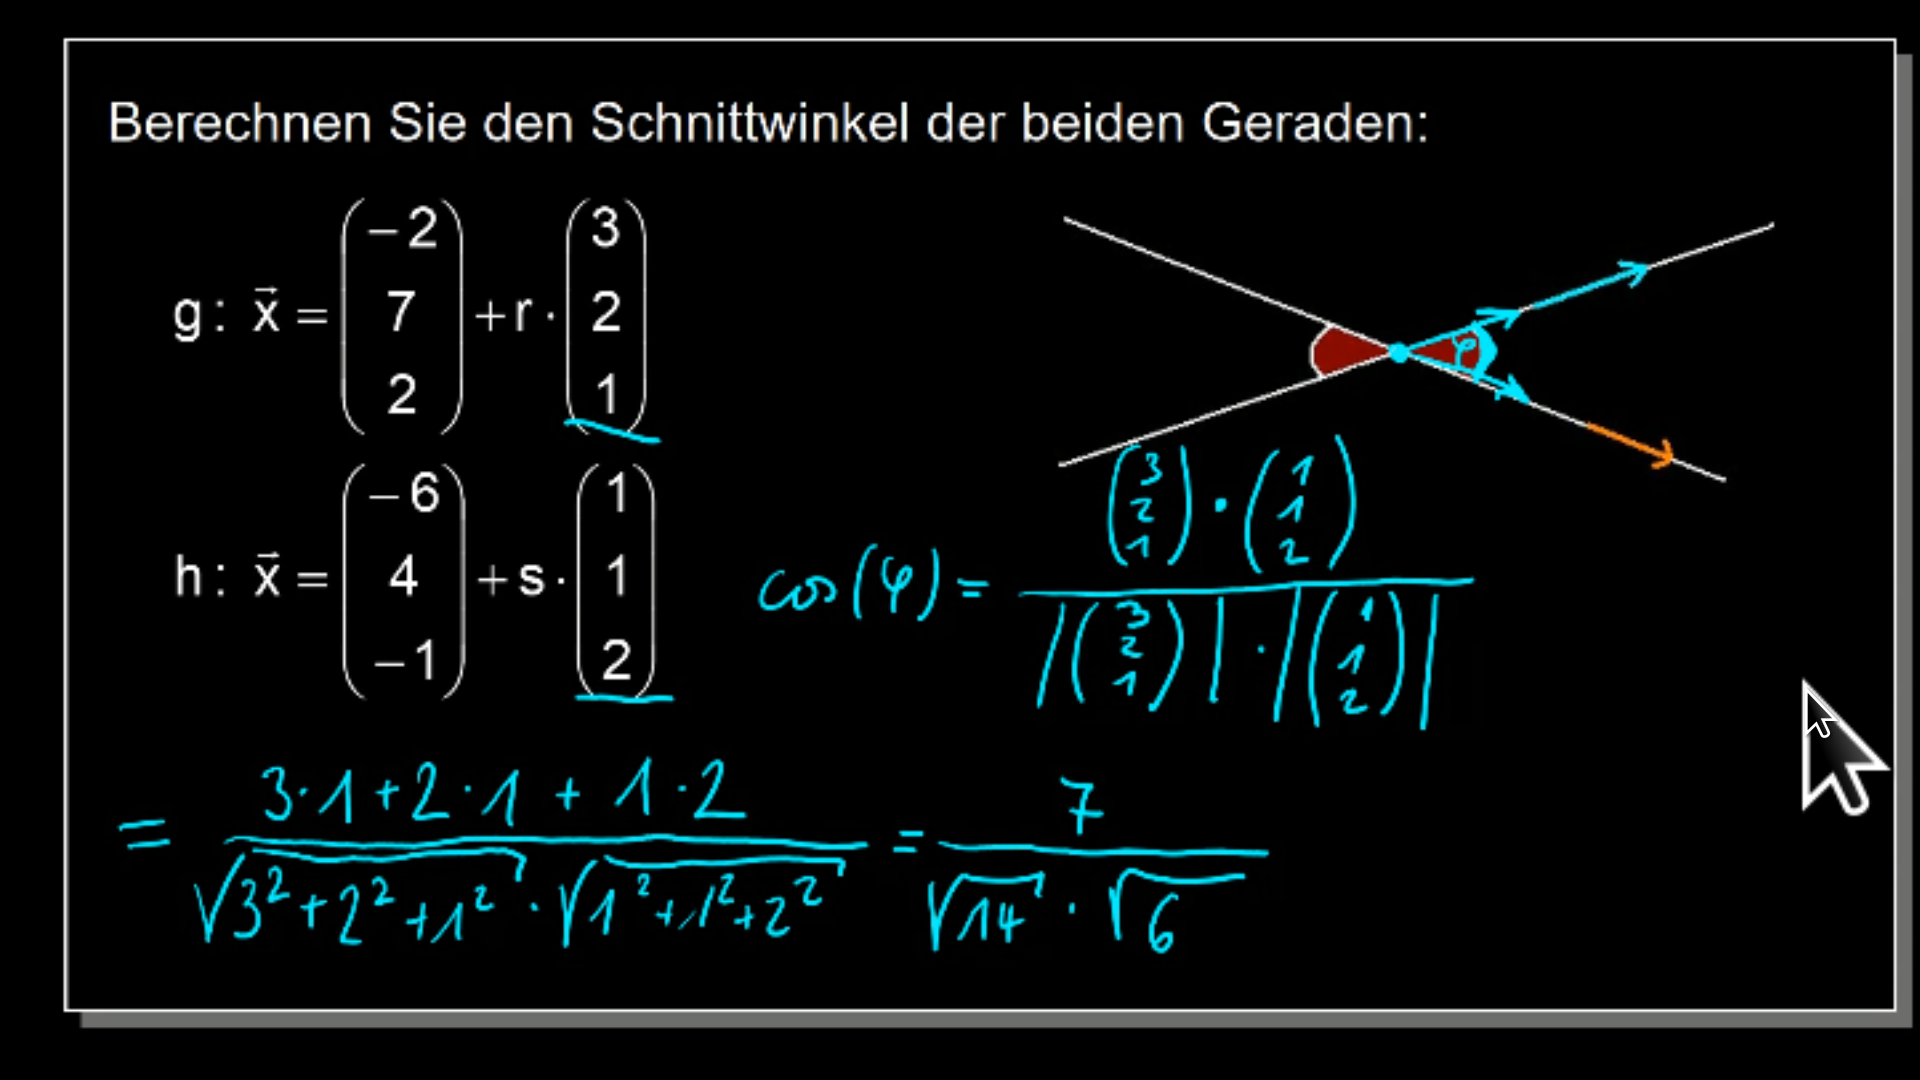
\includegraphics[width=\linewidth]{sampleWinkel}
	\\
	Wenn Skalarprodukt 0 dann WInkel zwischen Vektoren 90 Grad \\
	orthogonal \\
	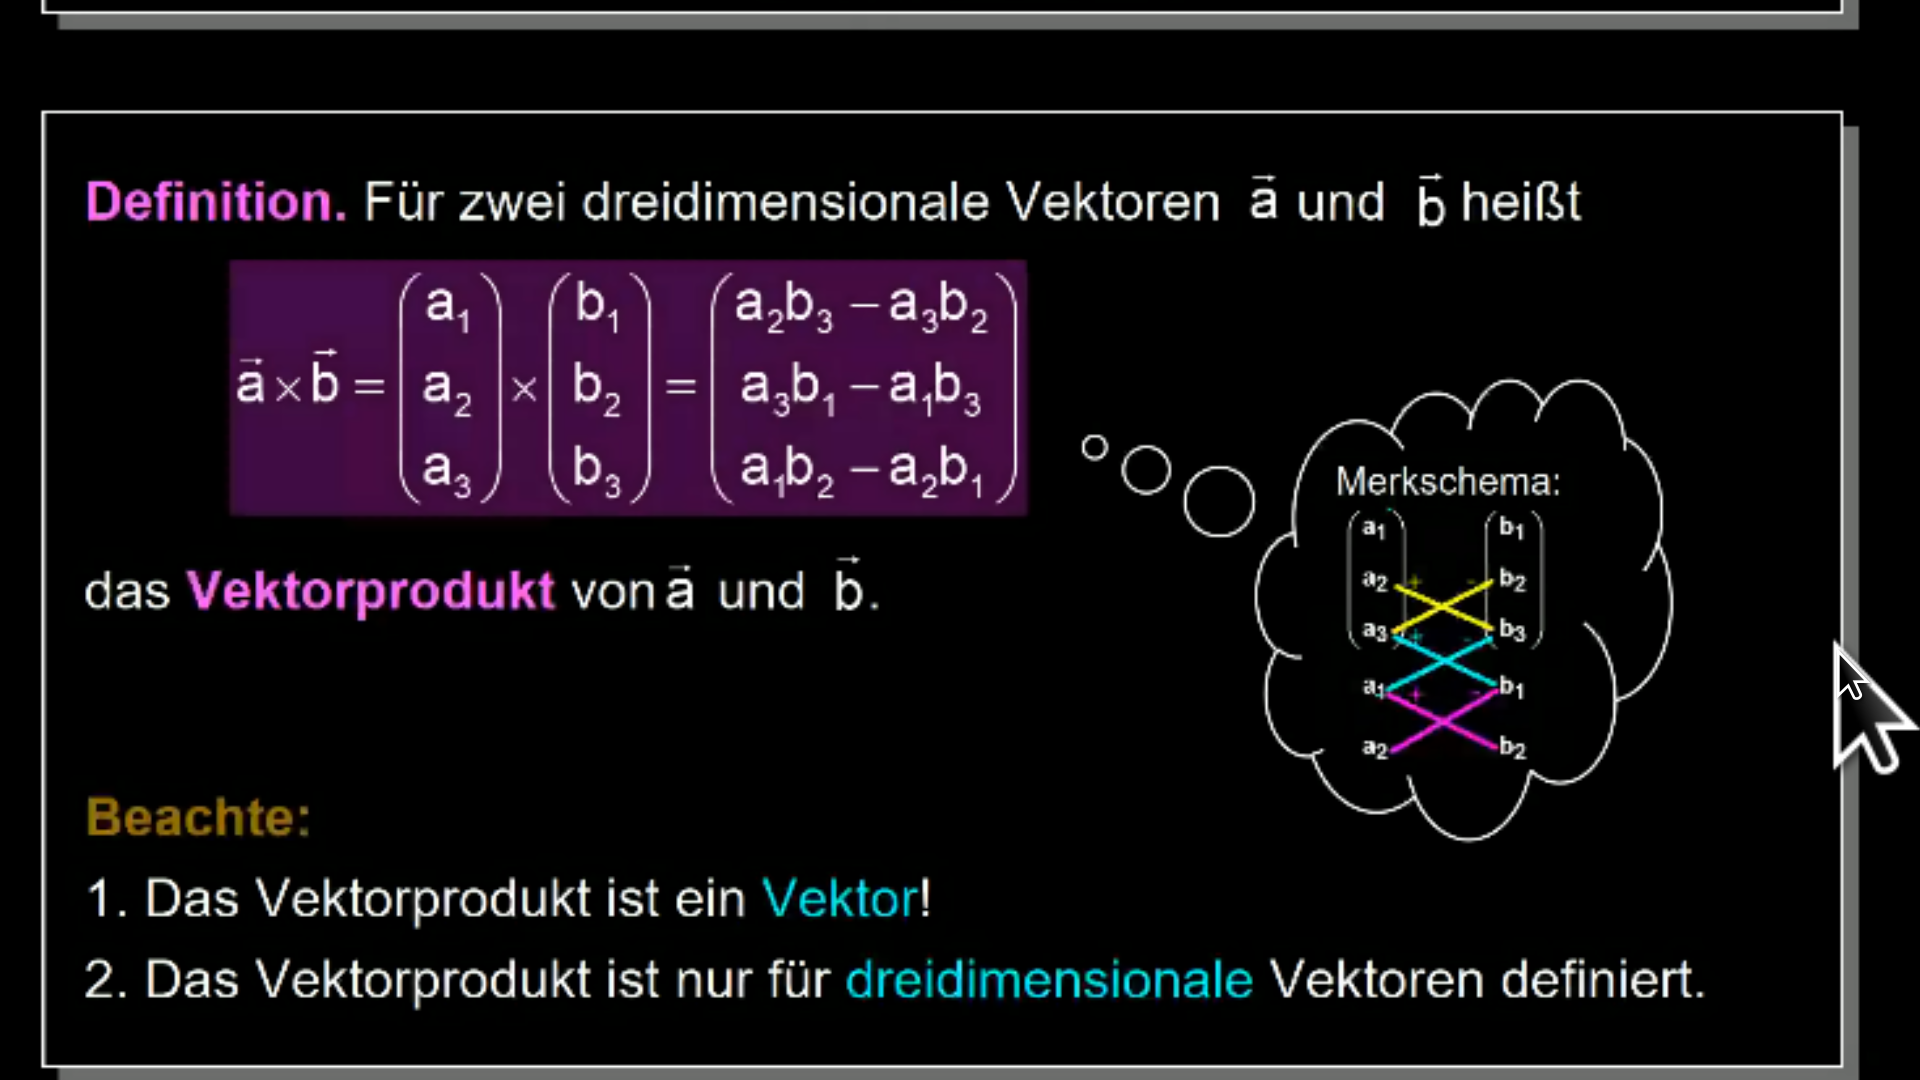
\includegraphics[width=\linewidth]{VecProd1} \\
	Vektorprodukt ist nur, und nur für 3 dimensionale Vektoren definiert. \\
	Vektorprodukt ist zu den Vektoren a und b senkrecht. \\
	Stichpunkt Normalenvektor der Ebene \\
	Vektorprodukt bedeutet geometrisch gesehen die Fläche eines Parallelogramms. \\
	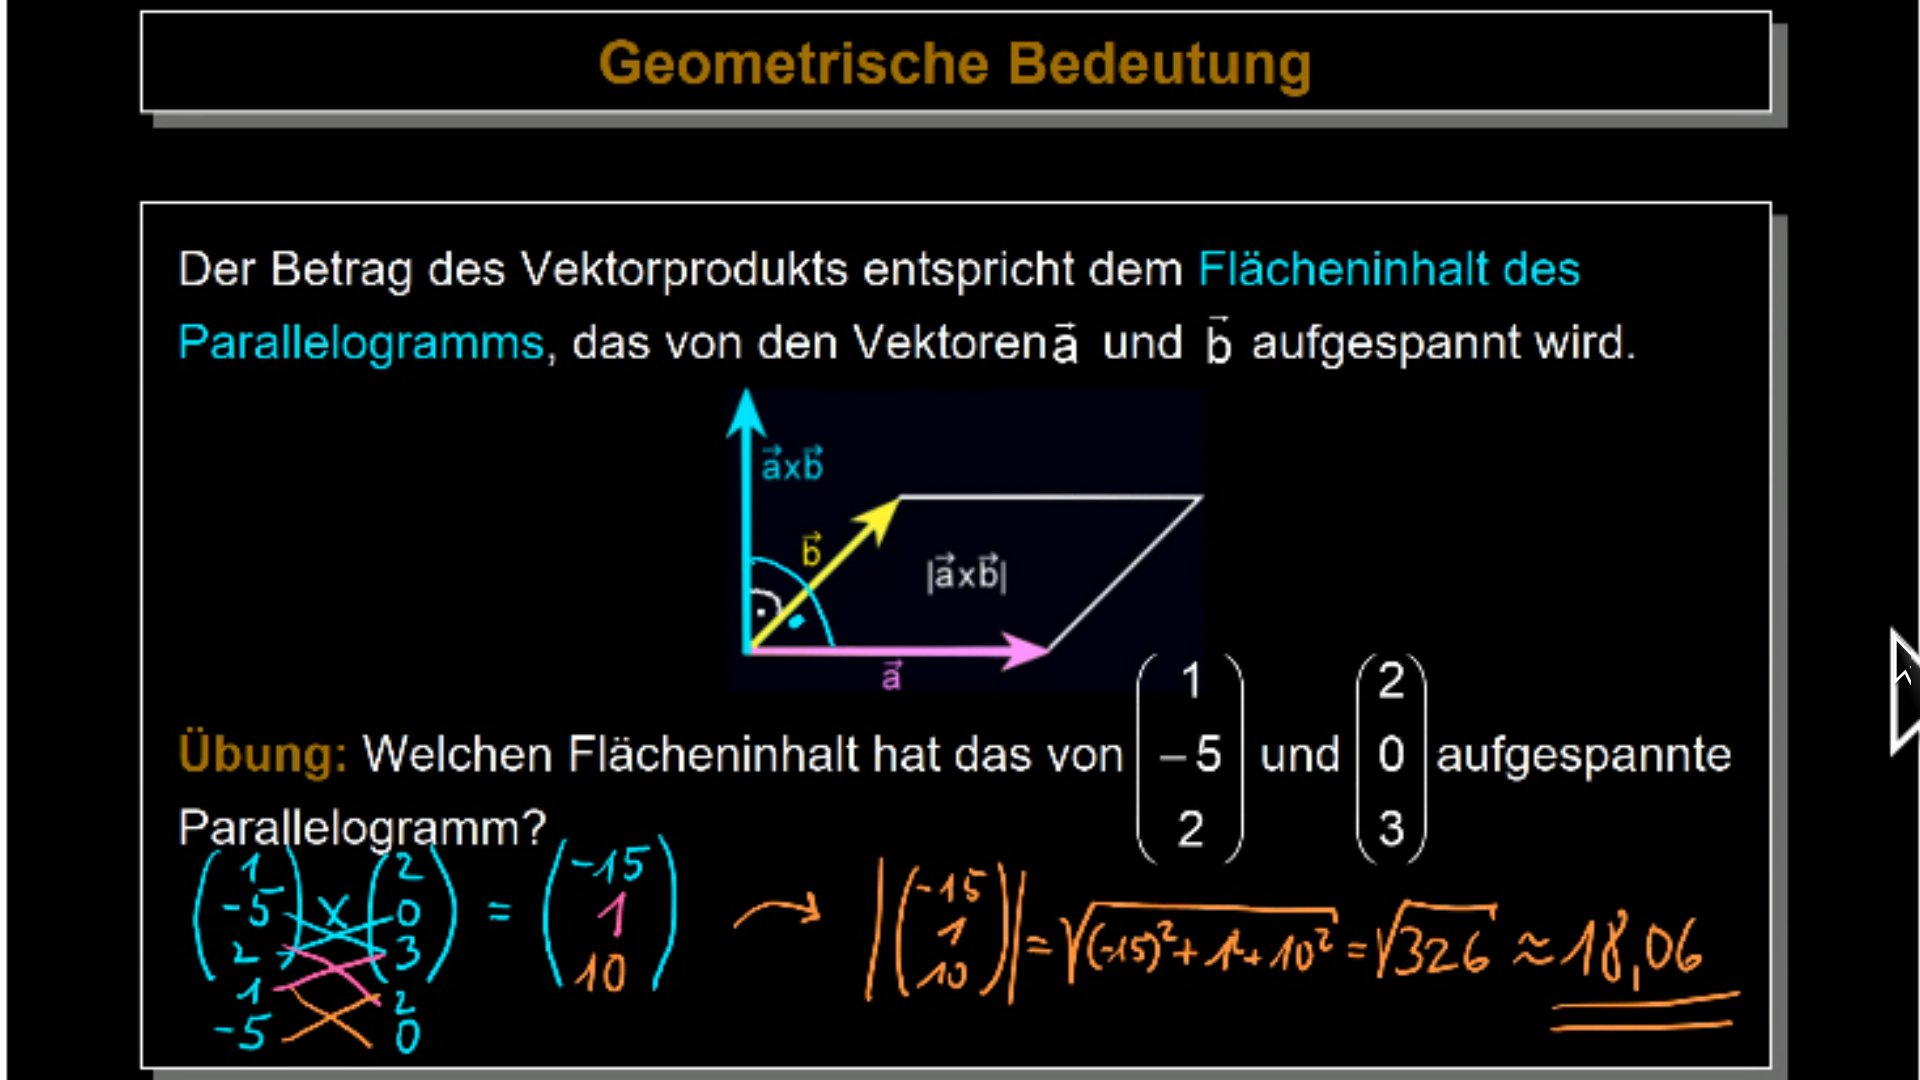
\includegraphics[width=\linewidth]{GVP} \\
	Für Dreieck das ganze * $\frac{1}{2}$ \\
	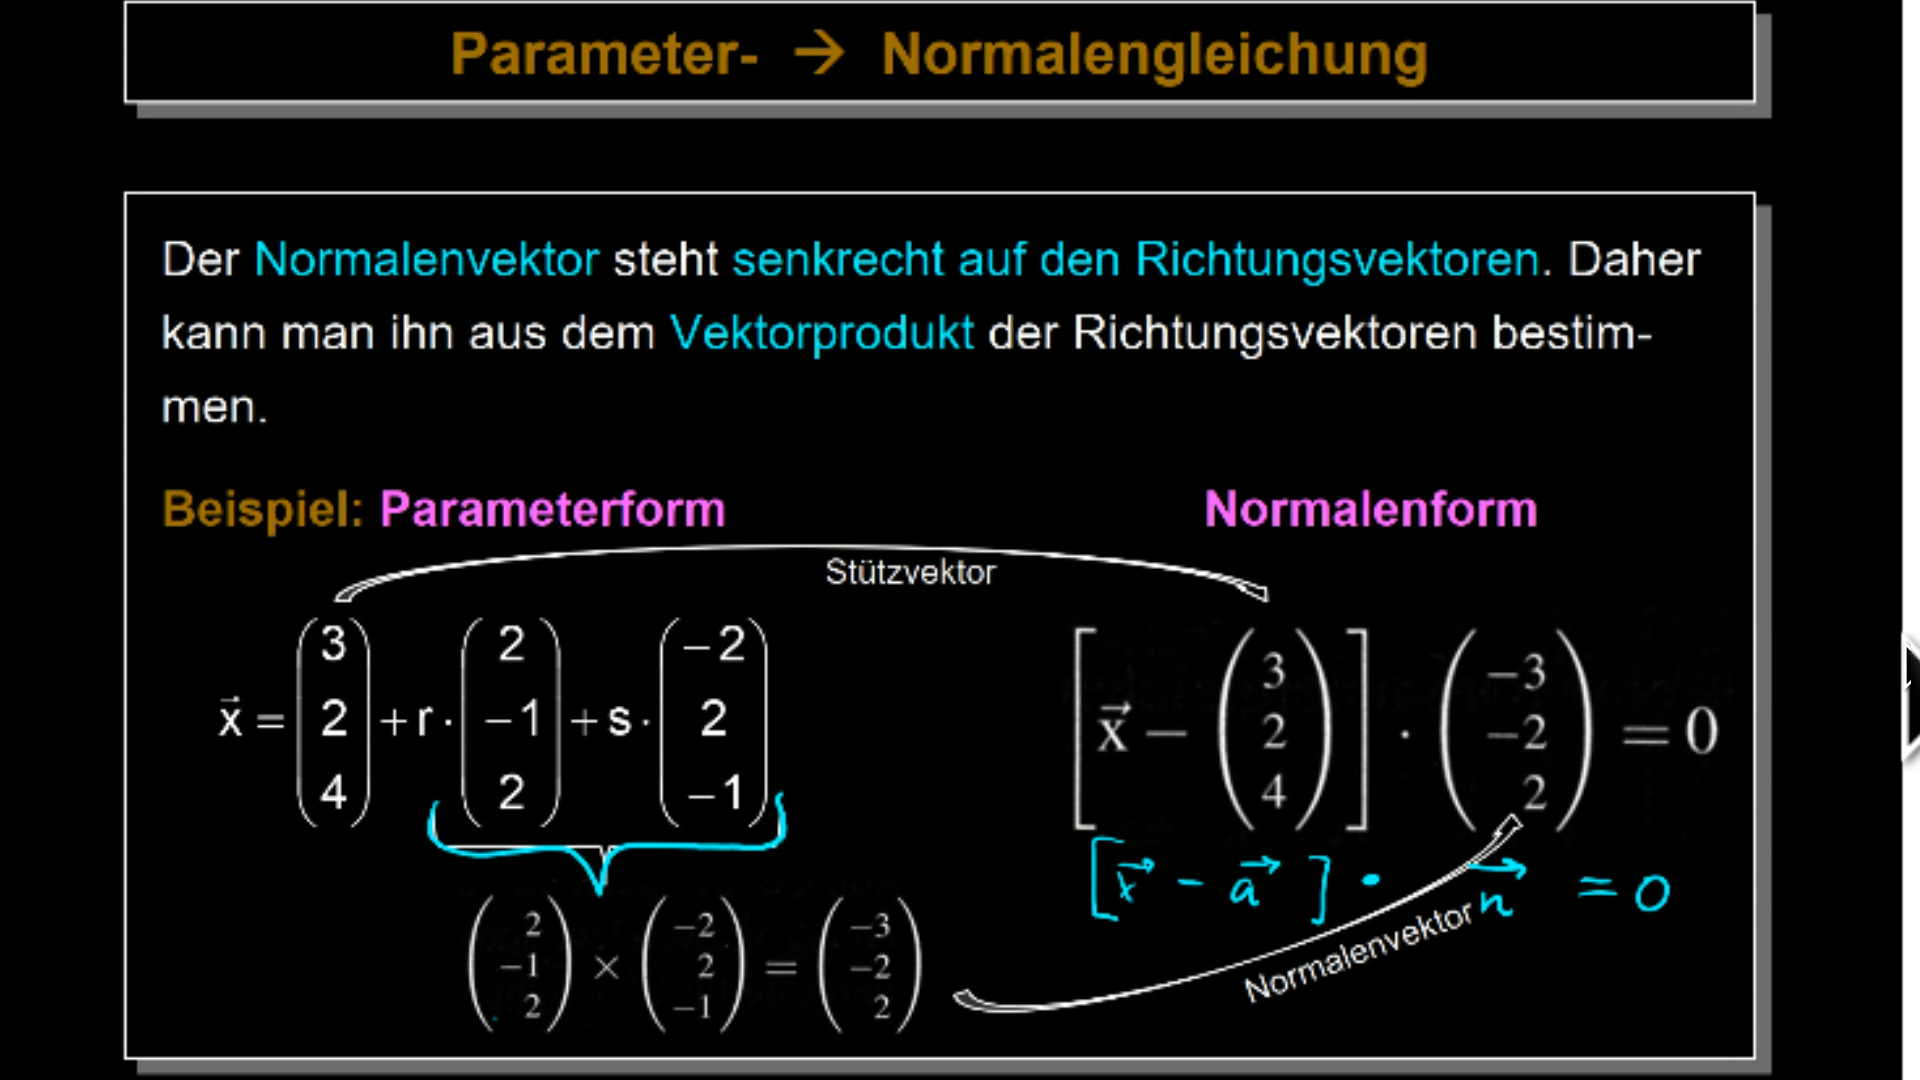
\includegraphics[width=\linewidth]{wechsel}
	Von NF auf Koordinatengleichung ausmultiplizieren. \\
	Schnittwinkel $\alpha$ = 90 - $\phi$ \\
	Winkel zwischen Ebenen ist Winkel zwischen Normalvektoren. \\
	Lotfußpunktverfahren \\
	liefert Abstand Punkt ebene \\
	Von einem Punkt fällt eine Gerade in die Ebene. \\
	Suche Durchstoßpunkt der Ebene. \\
	Berechne Betrag Vektor P,Durchstoßpunkt \\
	Hesse'sche Normalenform mit Normalvektor mit Betrag 1 \\
	Diese Form wird verwendet um Abstandsformel herleiten zu können \\
	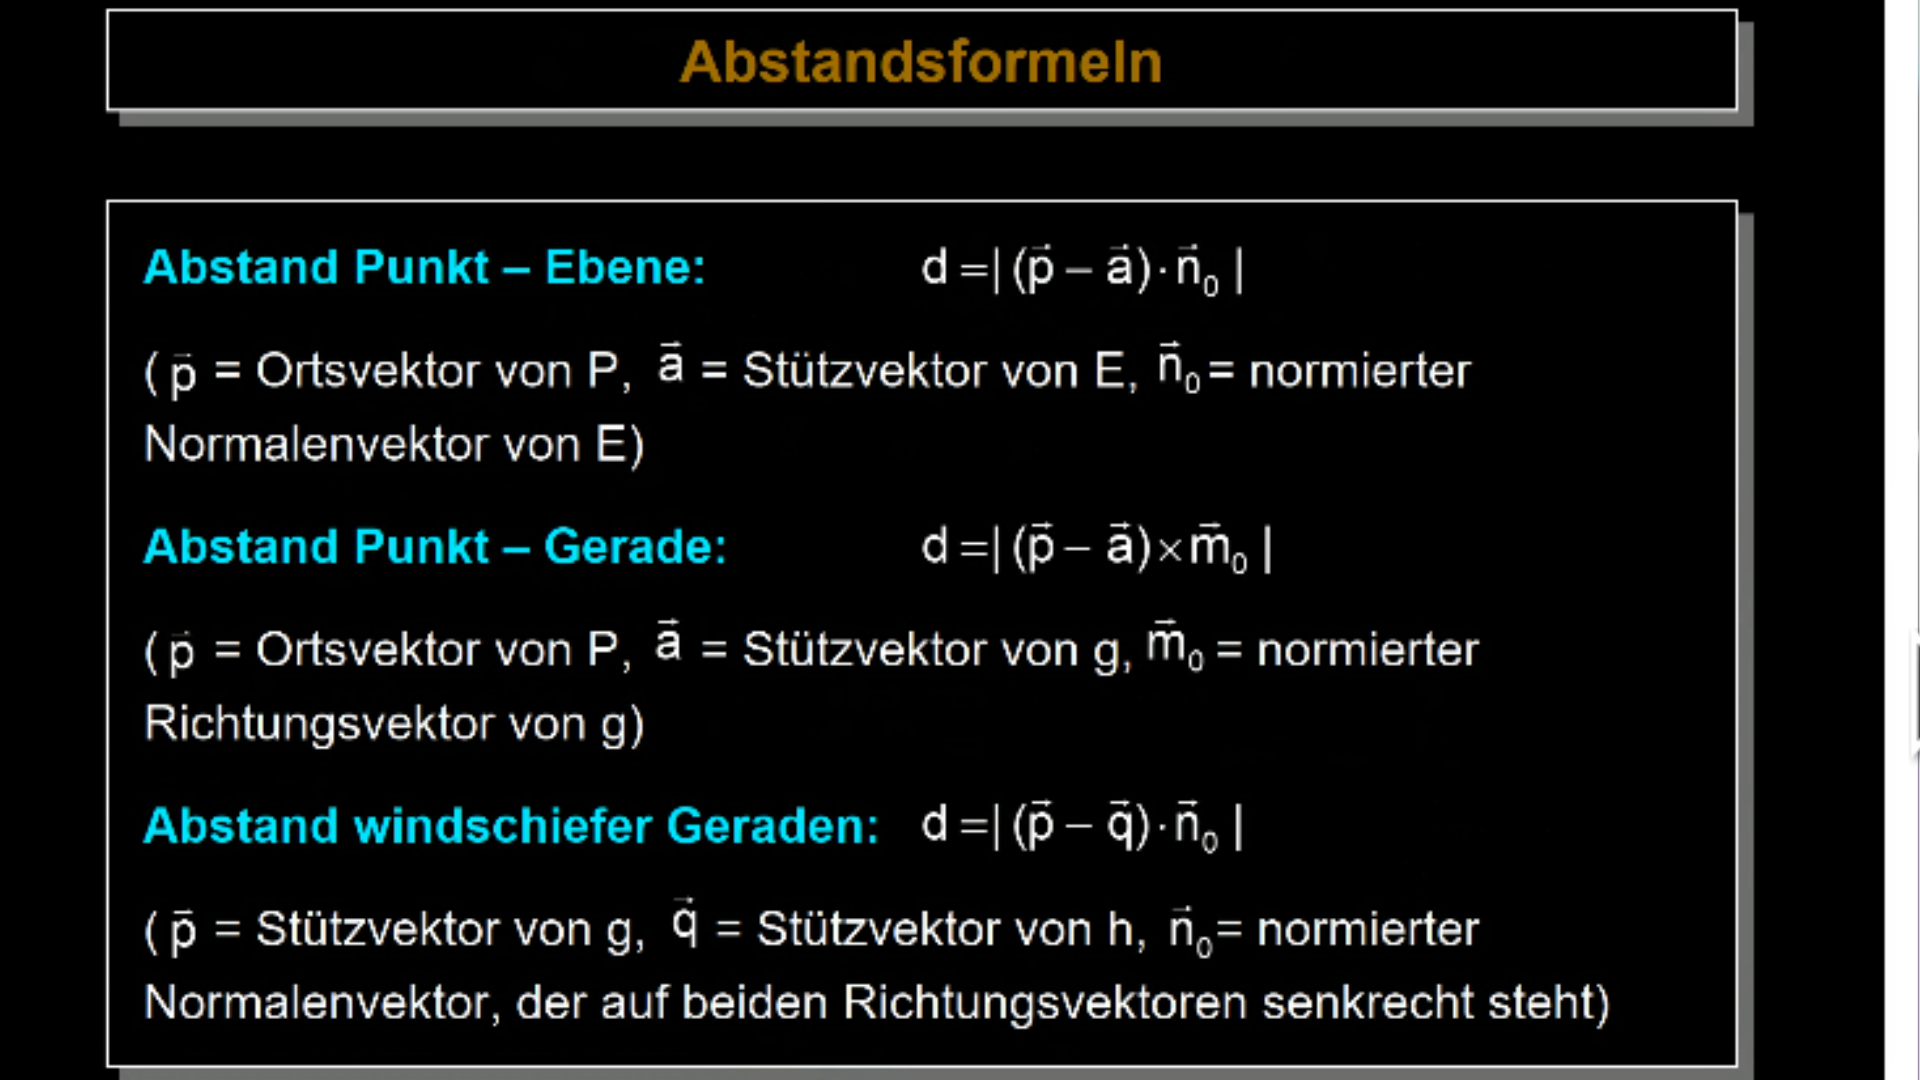
\includegraphics[width=\linewidth]{formeln}
	\subsection*{18.05.2021}
	Matrizen \\
	quadratische Matrix \\
	Matrizen können LGS lösen \\
	Vektoren = spezielle Matrizen \\
	Einheitsmatrix hat 1 in der Diagonalen. \\
	Stellt neutrales Element dar. \\
	Matrixaddition ähnlich Vektoraddition \\
	Matrixmultiplikation \\
	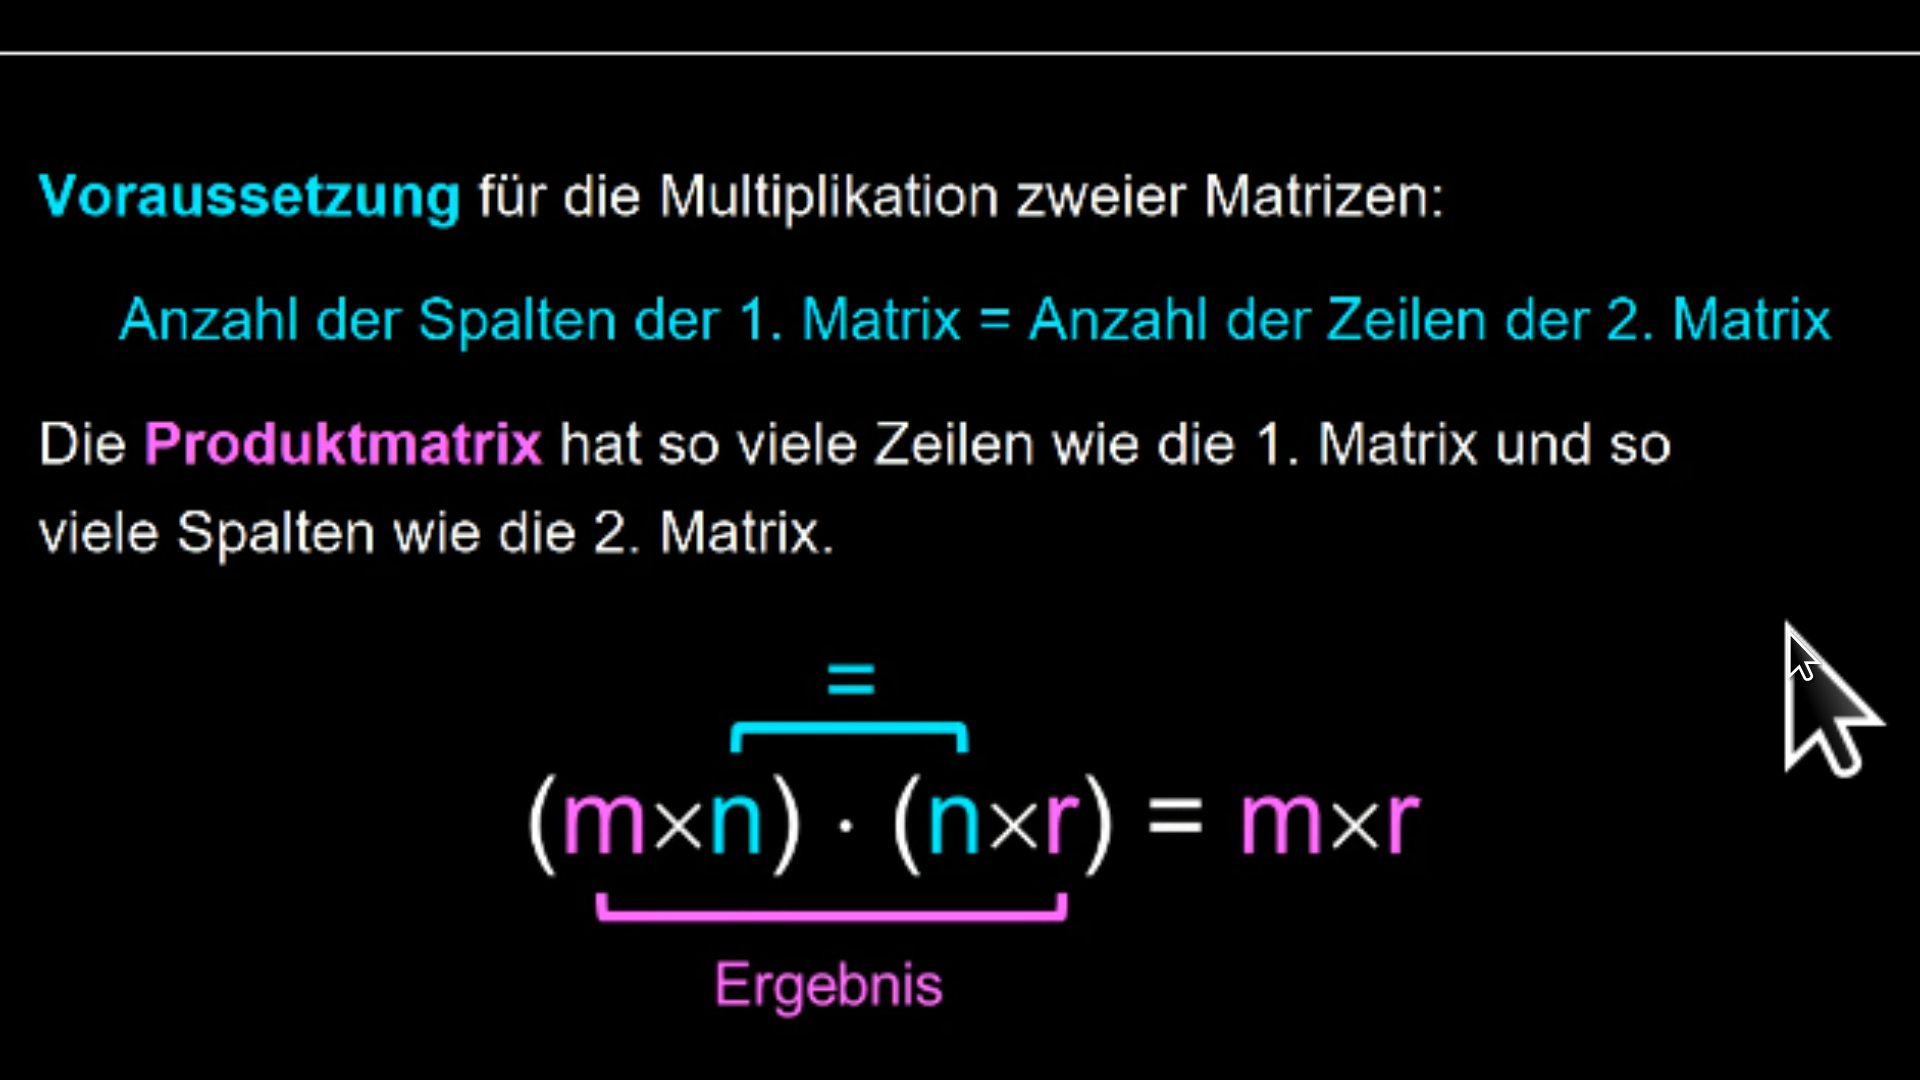
\includegraphics[width=\linewidth]{mat}
	Matrix 1 hat genauso viele Zeilen wie die zweite Matrix Spalten hat. \\
	Schema s.o. \\
	Rang der Matrix ist die Anzahl der linear unabhängigen Zeilen. \\
	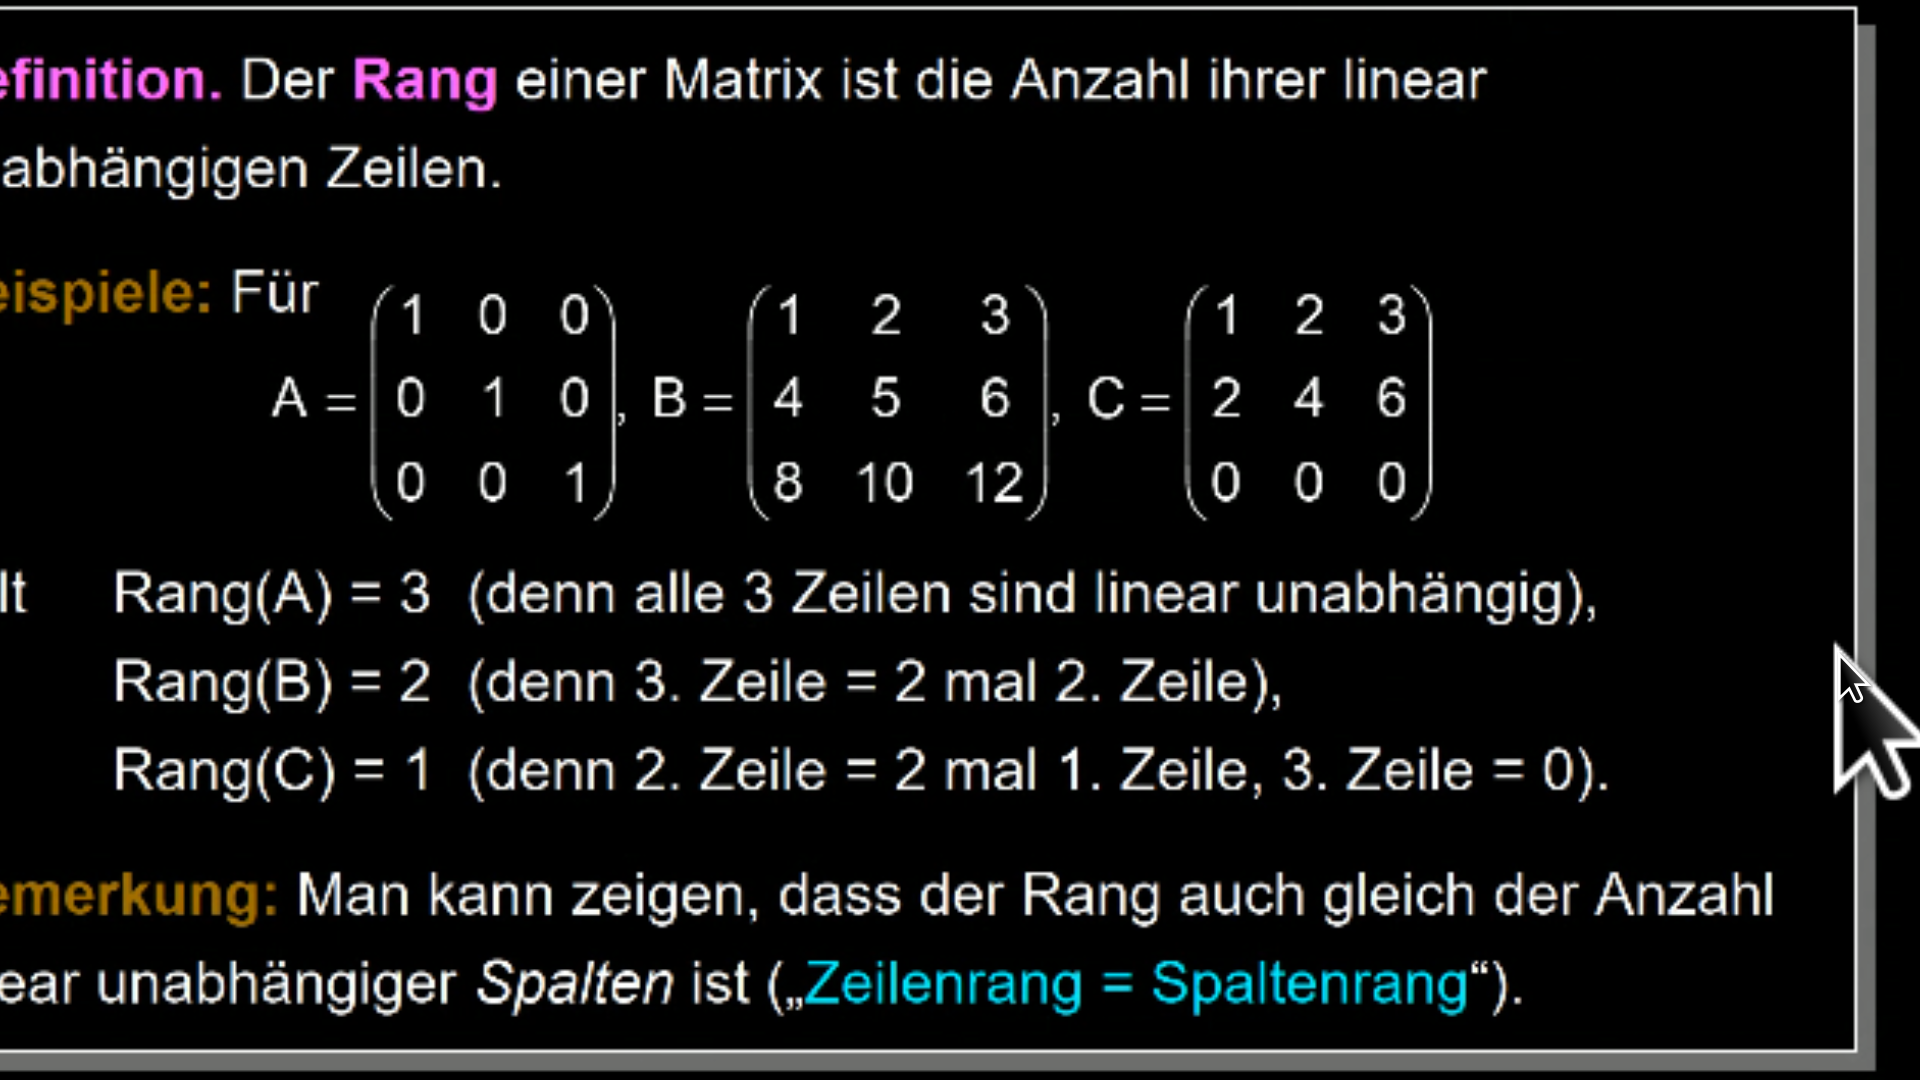
\includegraphics[width=\linewidth]{rang} \\
	A Rang = 3 \\
	B Rang = 2 \\
	C Rang = 1 \\
	Def. Der Rang einer Matrix ist die Anzahl ihrer linear unabhängigen Zeilen (oder Spalten).  \\
	Zeilenrang = Spaltenrang \\
	LGS mit Matrix: A $\cdot$ $\vec{x}$ = $\vec{b}$ \\
	Eindeutige Lösung wenn Matrix vollen Rang hat. \\
	A $\cdot$ $A^{-1}$ = E \\
	\subsection*{25.05.2021}
	Anwendung von Matrizen \\
	orthogonale Matrizen. \\
	Def. Inverse der Matrix muss gleich der transponierten Matrix sein. \\
	Transponieren = Spalten und Zeilen vertauschen. \\
	Um eine Matrix zu invertieren muss diese mit der transponierten Matrix multipliziert werden. \\
	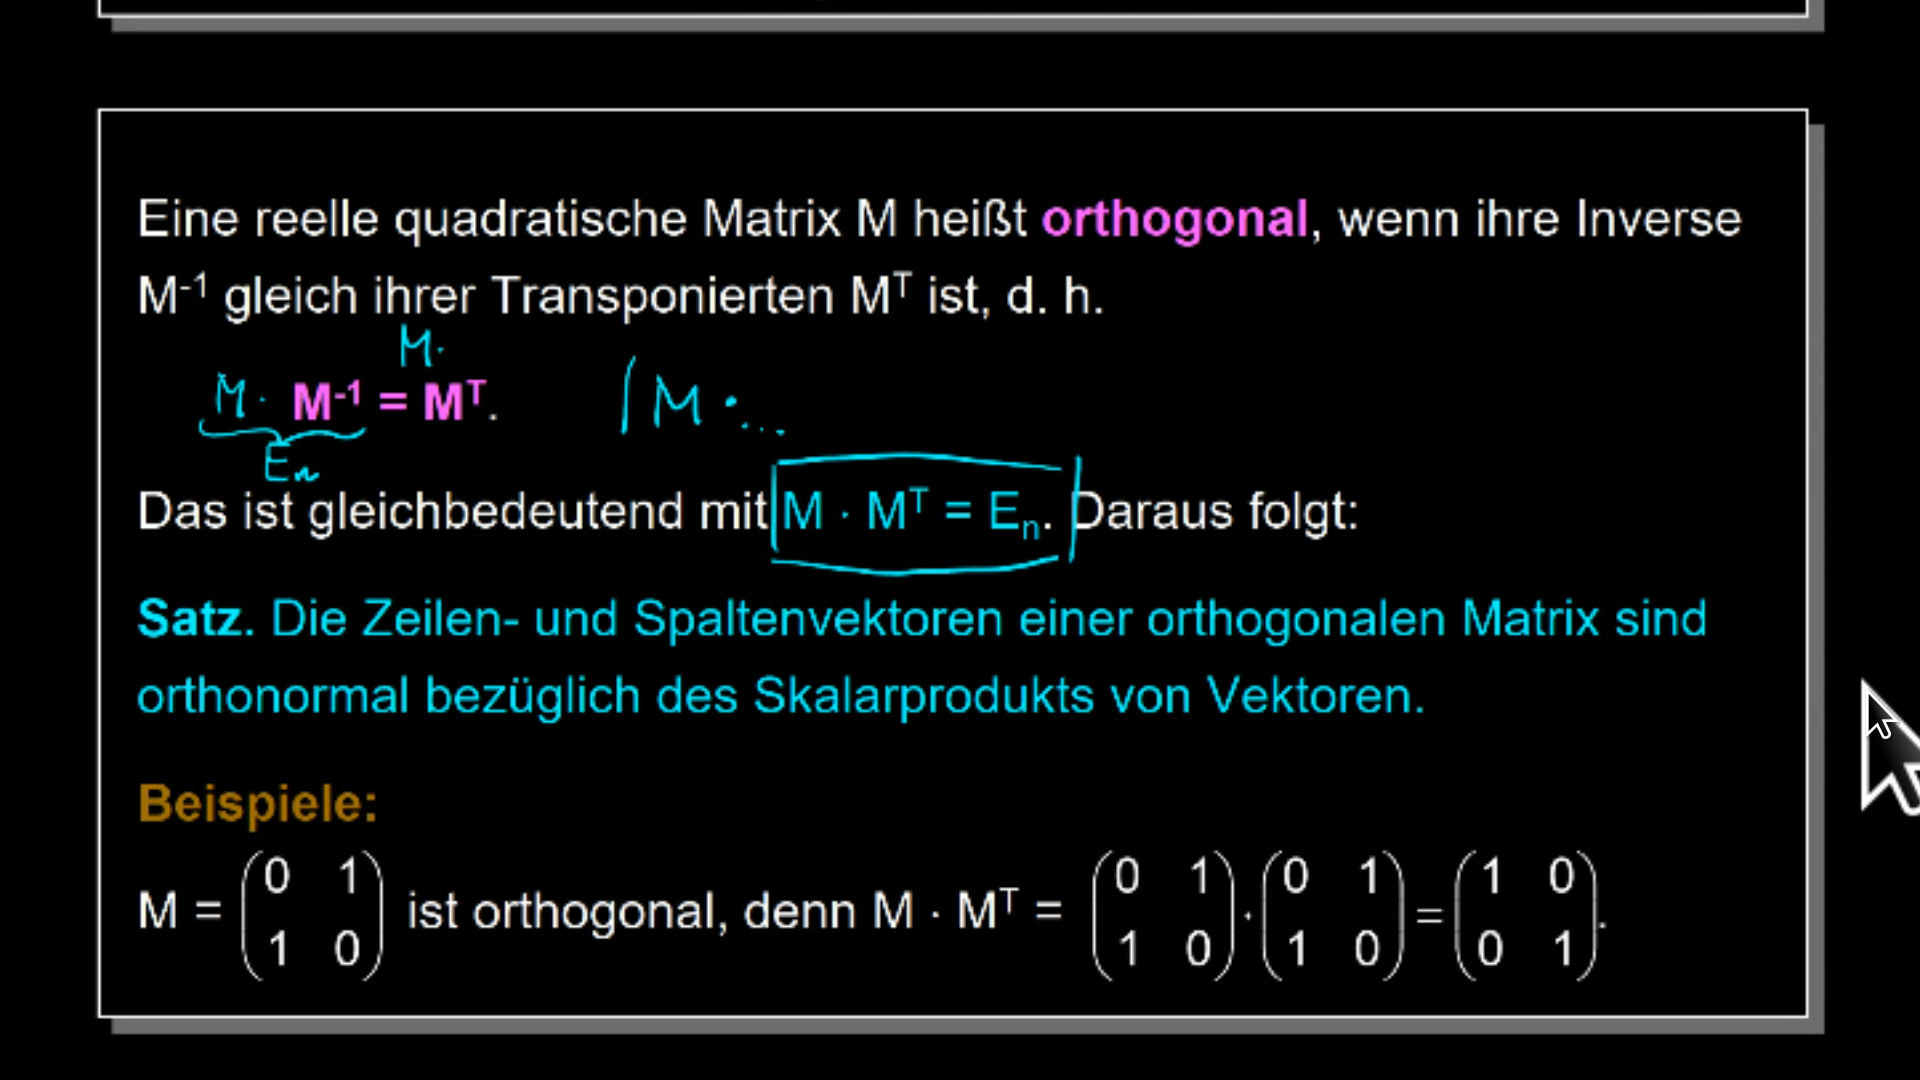
\includegraphics[width=\linewidth]{tanspo} \\
	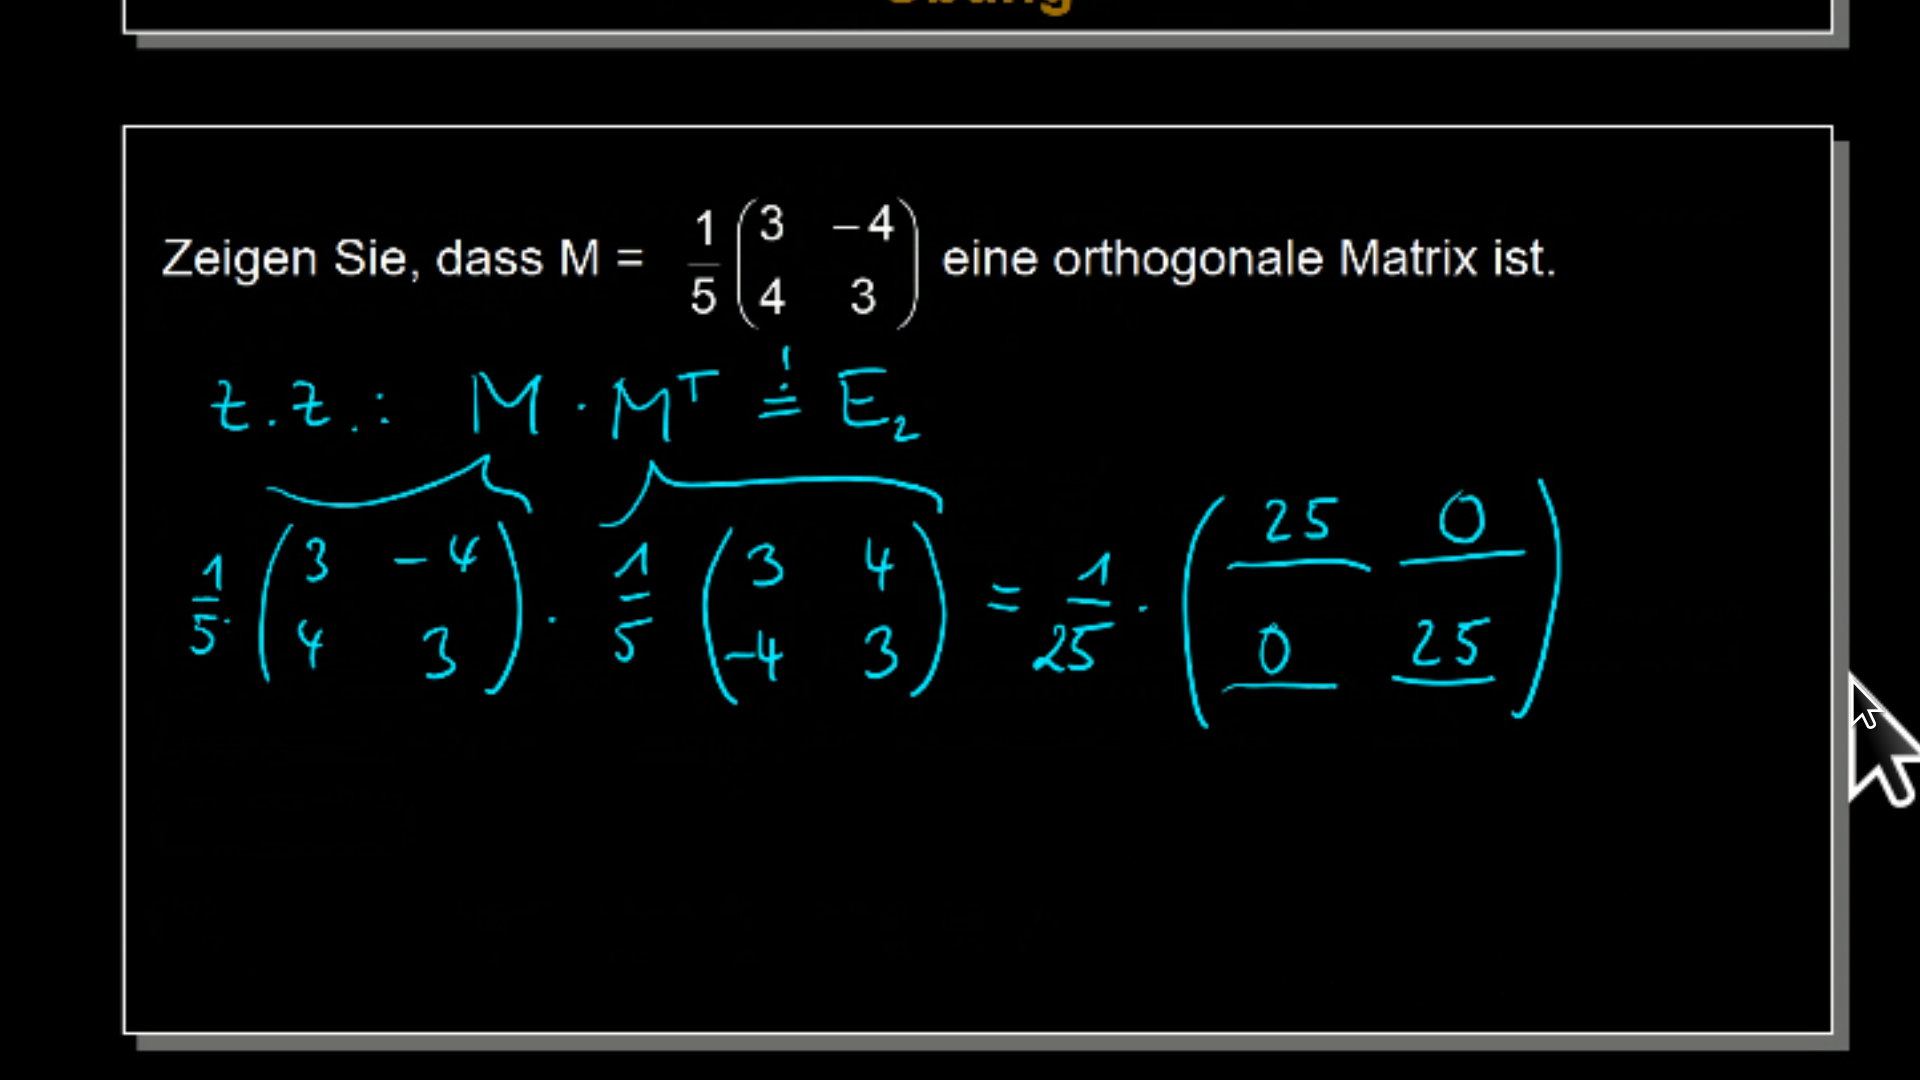
\includegraphics[width=\linewidth]{sample2} \\
	Beispielaufgabe aus der Vorlesung  \\
	Rohstoffsbedarfsmatrix \\
	Bedarfsvektor beachten \\
	\includegraphics[width=\linewidth]{übungbedarf} \\
	Aufgabe aus der Vorlesung \\
	\includegraphics[width=\linewidth]{übedarfsolv} \\
	Lösung für die Übung aus der Vorlesung. \\
	Übergangsmatrix $\cdot$ Anfangszustand = Folgezustand \\
	Irgendwann ändert sich der Folgezustand nicht mehr. \\
	jede stochastische Matrix hat einen Vektor mit stabilem Zustand. \\
	Es gibt genau einen Fixvektor \\
	Solange der Startzustand $\neq$ 0 streben die Folgezustände gegen den Fixvektor \\
	Determinanten \\
	Determinanten sind Zahlen die einer Matrix zugeordnet werden \\
	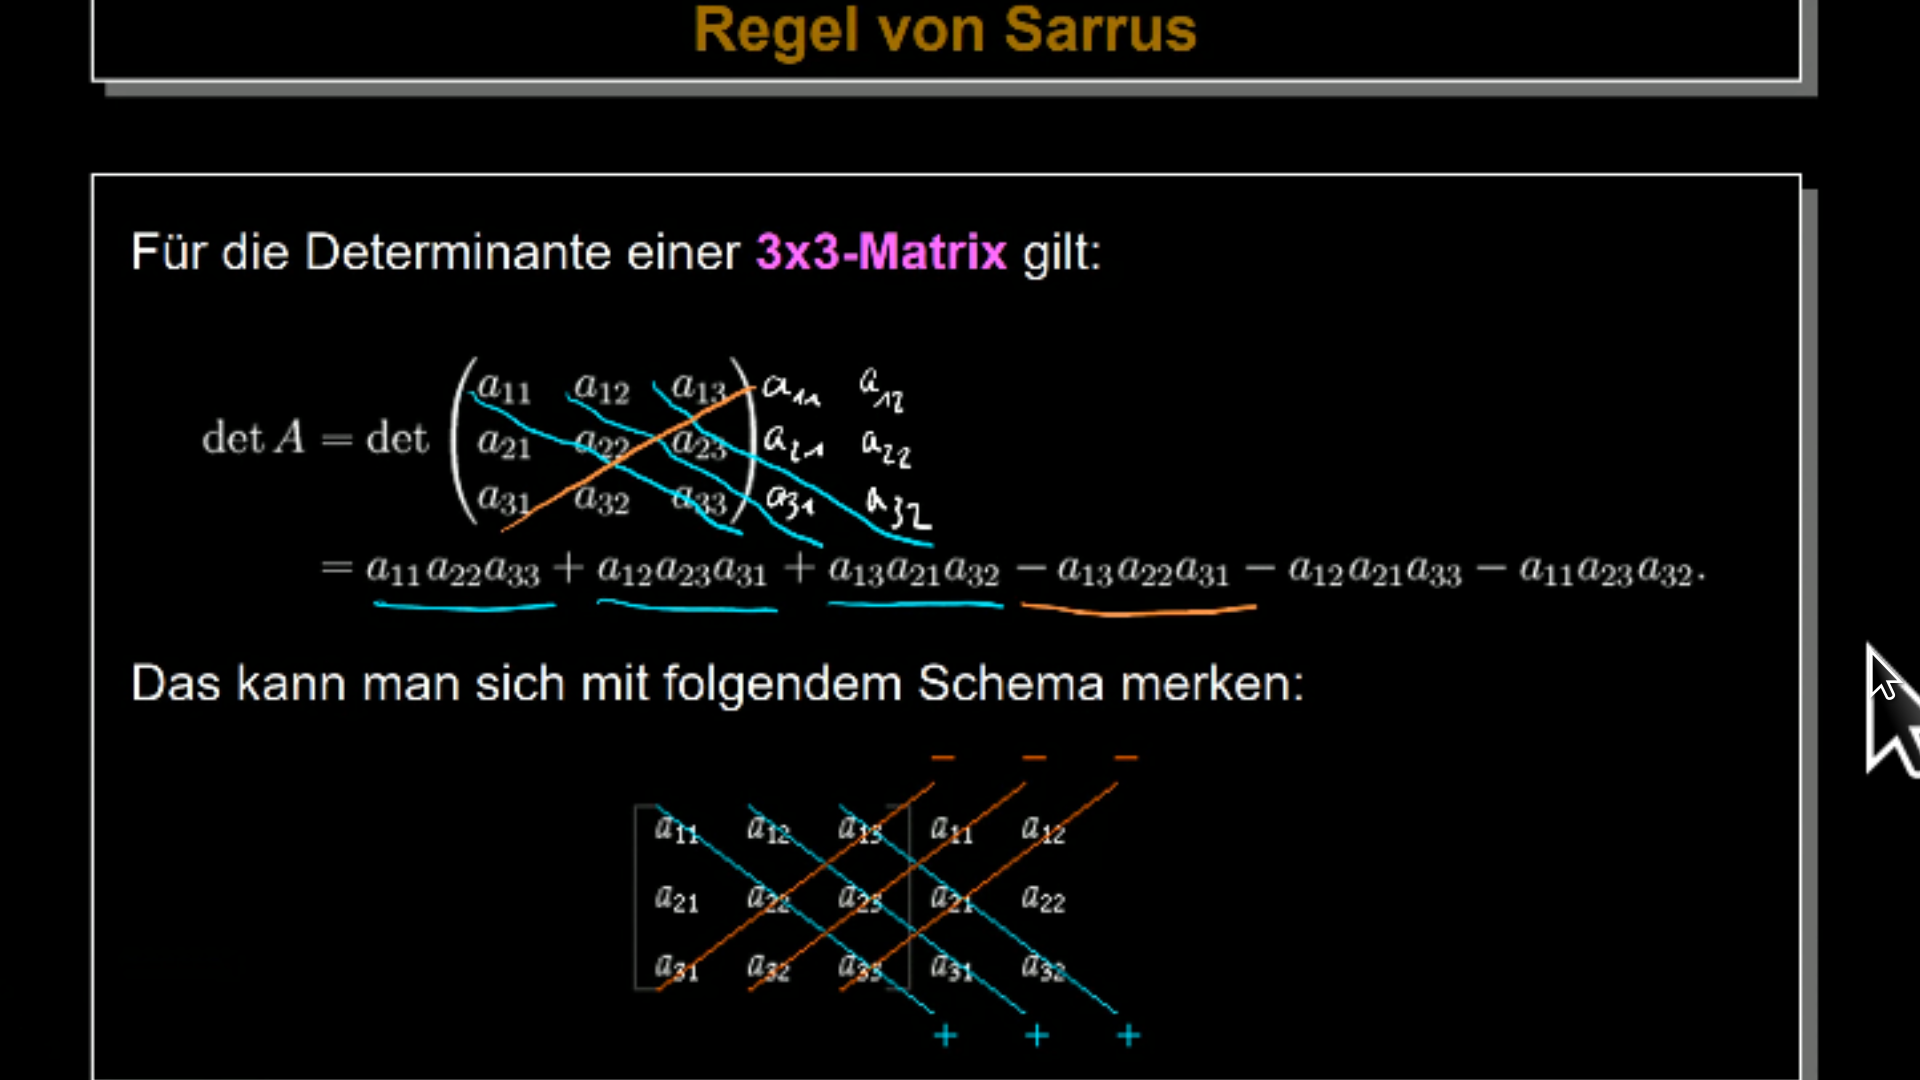
\includegraphics[width=\linewidth]{sarrus}\\
	Regel von Sarrus um Determinante zu berechnen. \\
	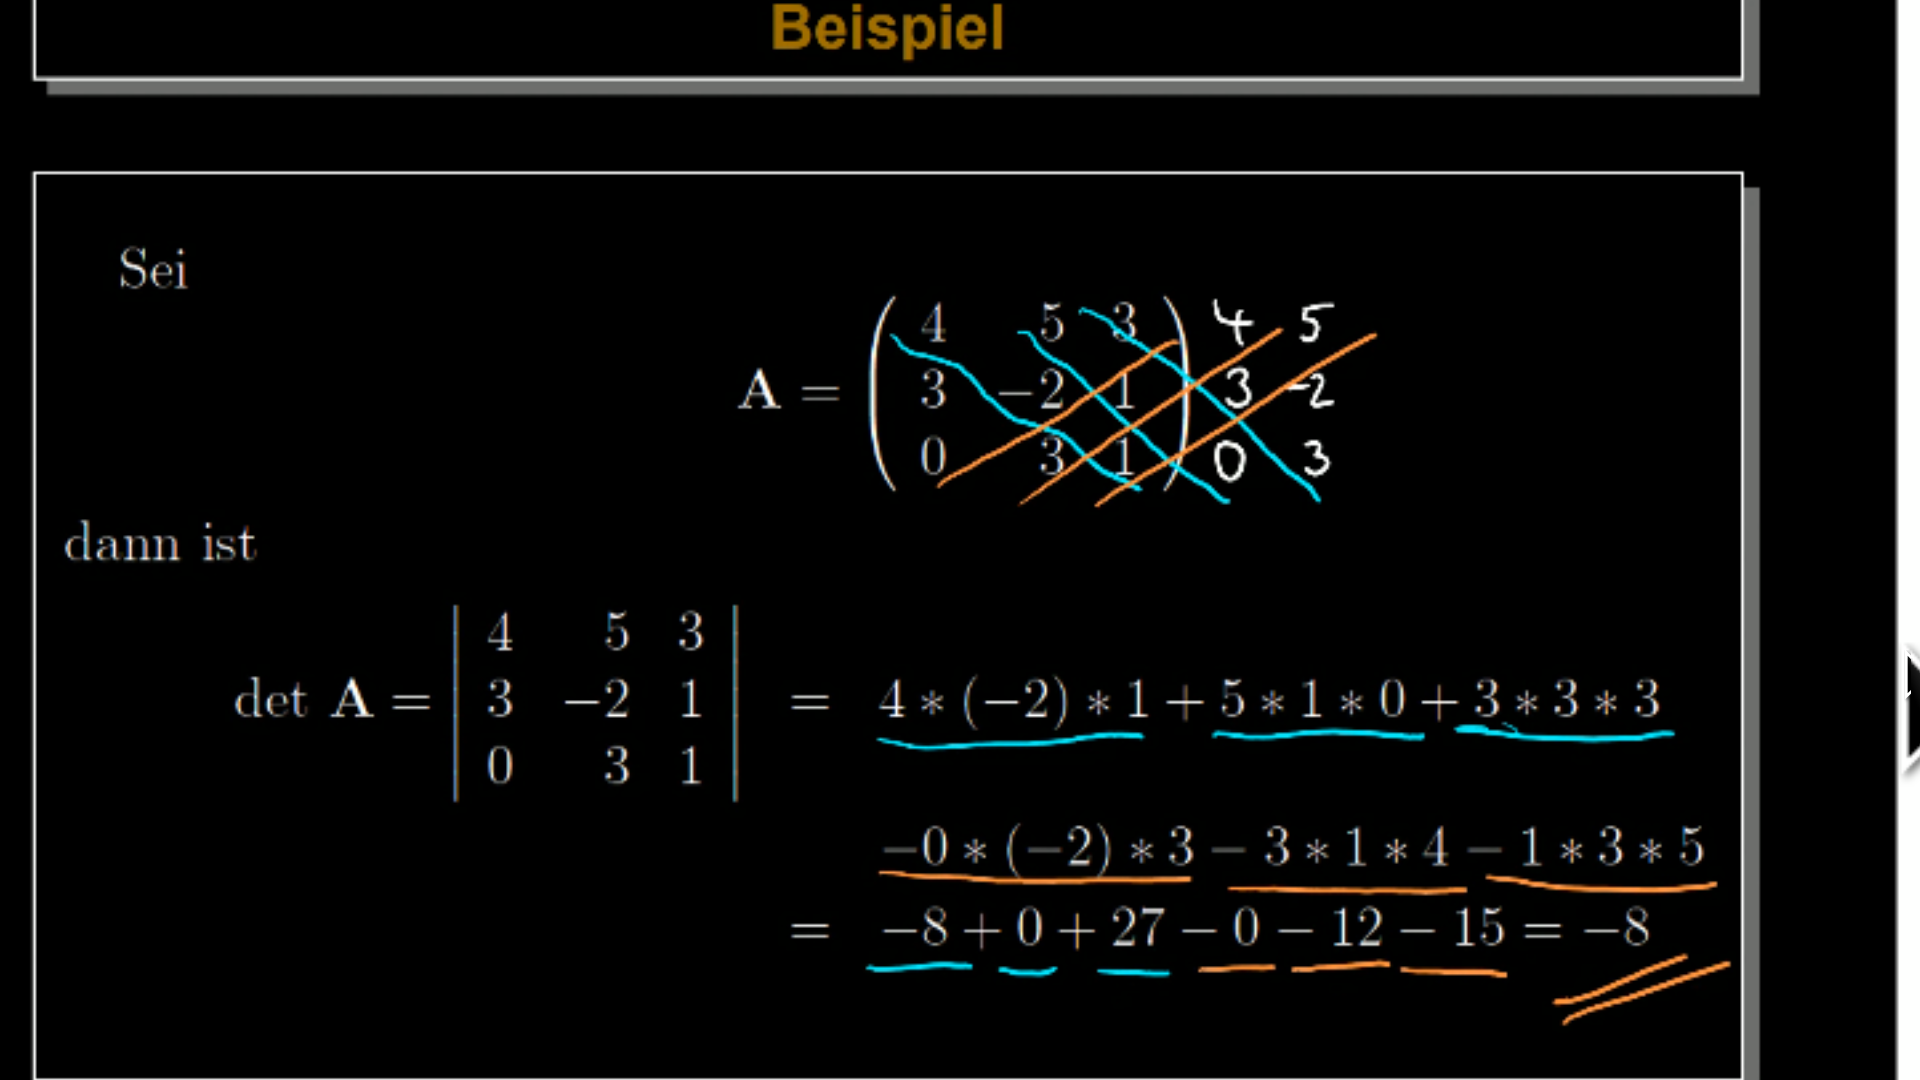
\includegraphics[width=\linewidth]{bsarrus} \\
	Beispiel für die Regel von Sarrus \\
	Gilt nur für 3 X 3 Matrizen \\
	\subsection*{01.06.2021}
	Determinante 2x2 entspricht Fläche des aufgespannten Parallelogramms. \\
	wichtig Betrag!!! \\
	2d Determinante = 0 bedeutet Fläche = 0; in 3D Volumen = 0 \\
	Wenn Vektoren linear abhängig, Determinante = 0 \\
	Determinante $\neq$ 0, Matrix ist invertierbar \\
	Cramersche Regel \\
	Kapitel 4 Lineare Abbildungen \\
	Matrix zur Abbildung Abbildung zur Matrix  \\
	Drehung, Streckung, Spiegelung  und Projektion in 2d und 3d \\
	Ansatz: \\
	$\vec{x'}$ = $\left(\begin{array}{cc}
	a & b \\ c & d
	\end{array}\right)$ $\cdot$
	$\vec{x}$ \\
	Matrixgleichungg \\
	kan in LGS umgewandelt werden oder aus LGS entwickelt werden. \\
	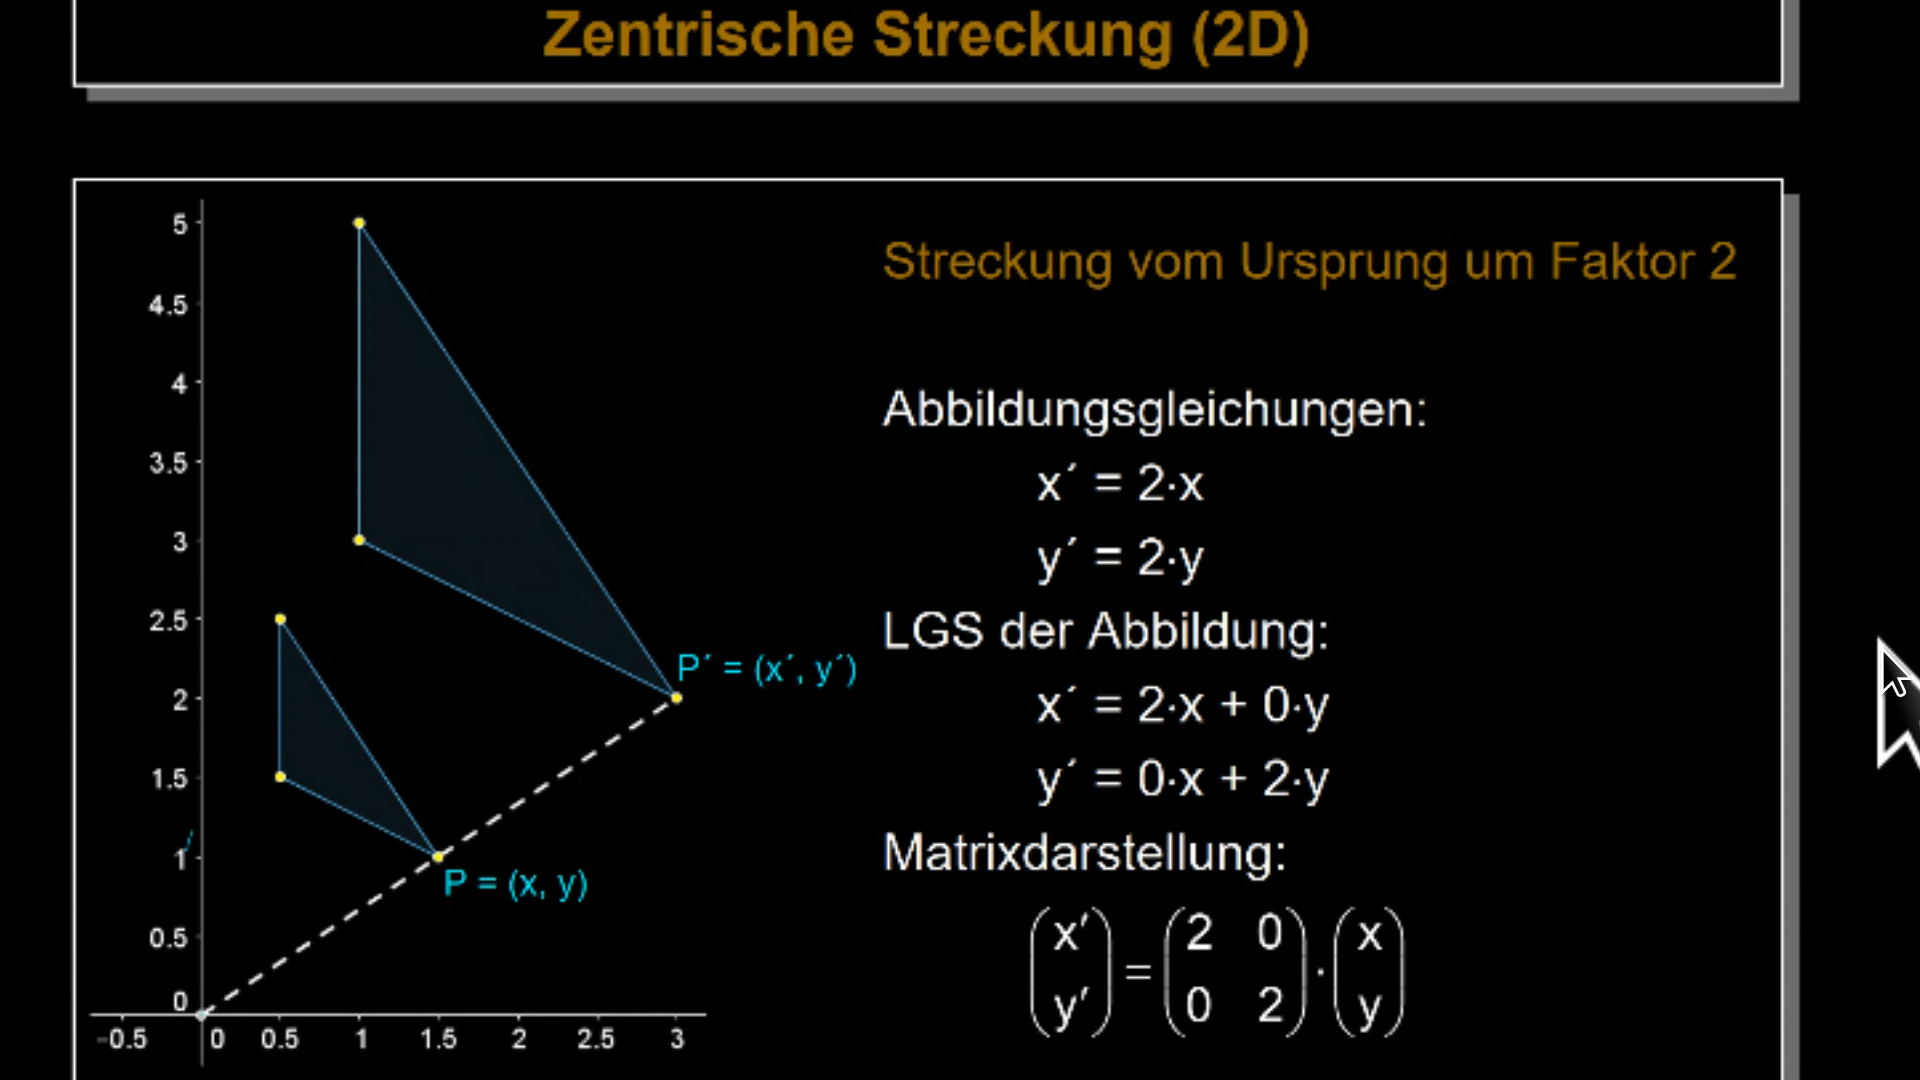
\includegraphics[width=\linewidth]{zstreckung} \\
	zentrische Streckung \\
	Streckmatrix merken: Einheitsmatrix $\cdot$ Streckfaktor \\
	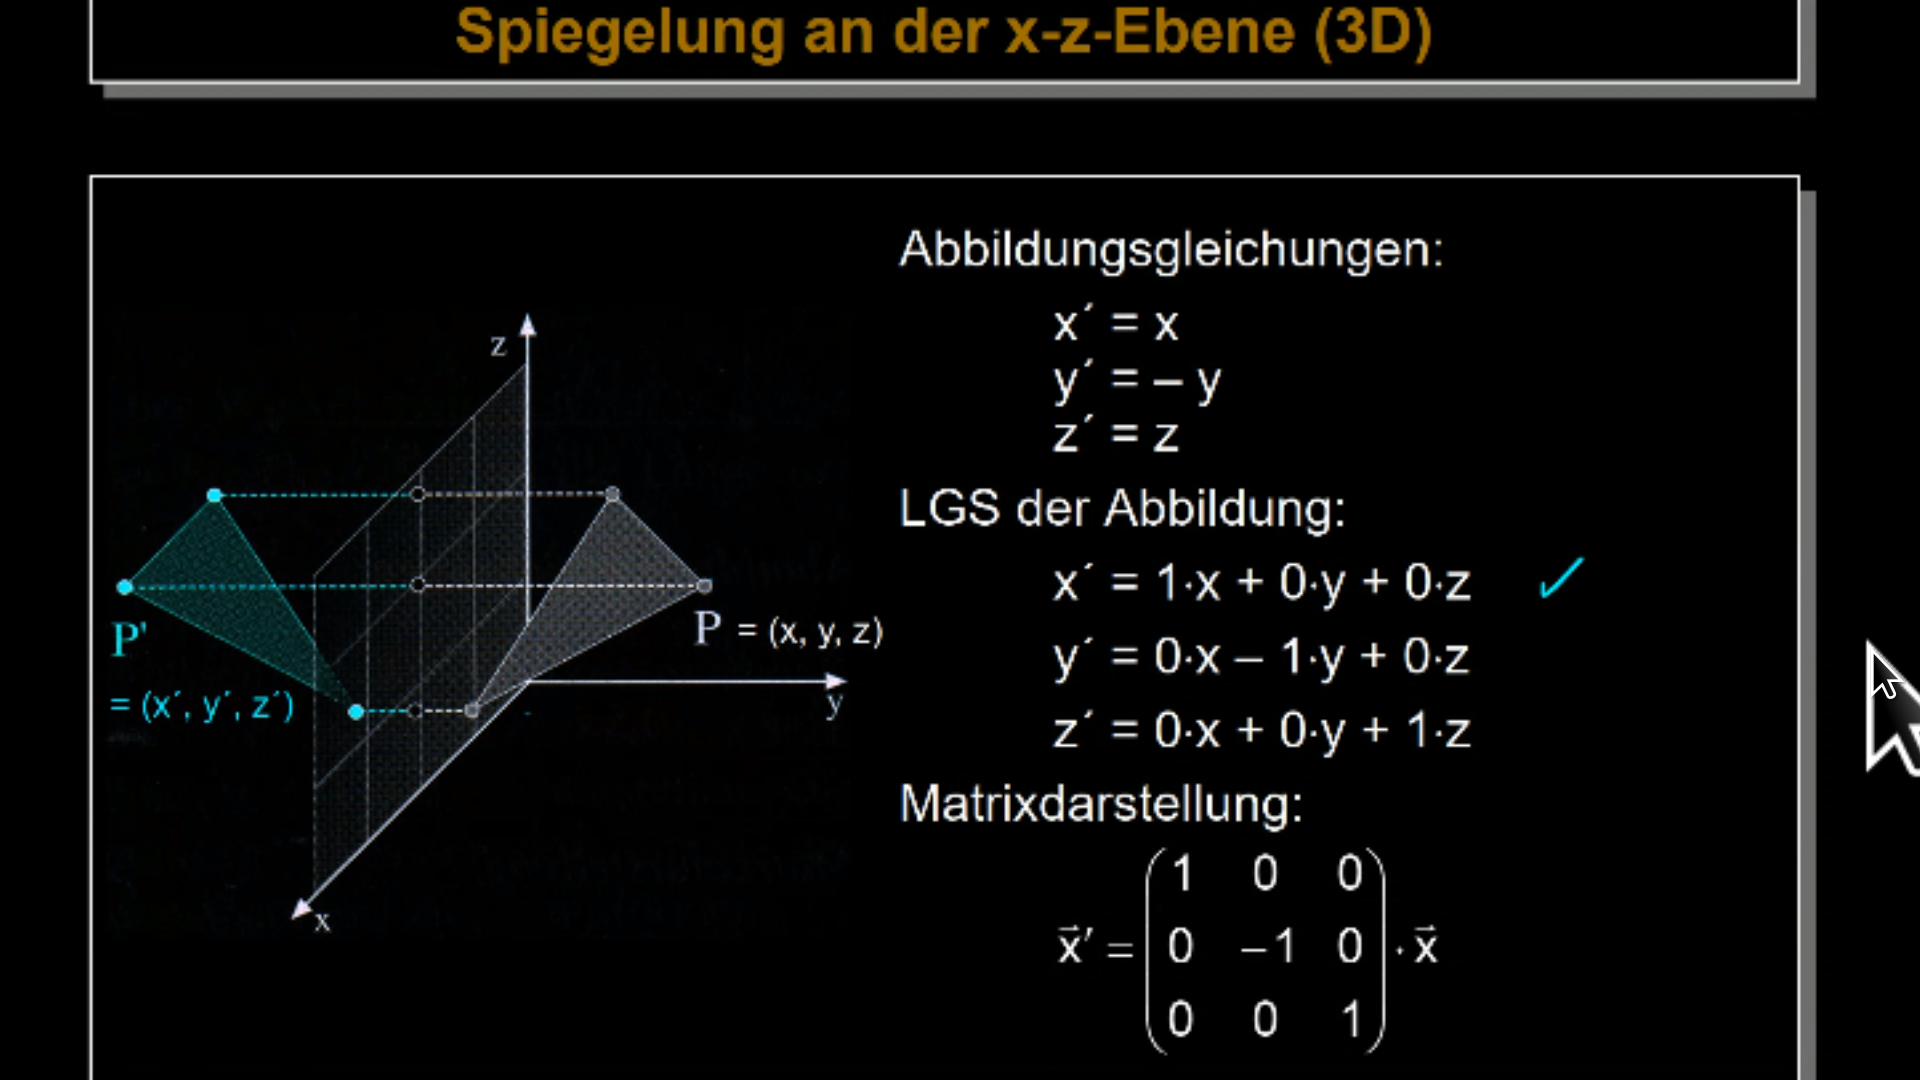
\includegraphics[width=\linewidth]{zes} \\
	Spiegelung an der x-z-Ebene \\
	Wichtig Höhe(z) ändert sich nicht y wird zu -y. \\
	Projektion \\
	Beispiel mit dem Schattenwurf auf die x-y-Ebene \\
	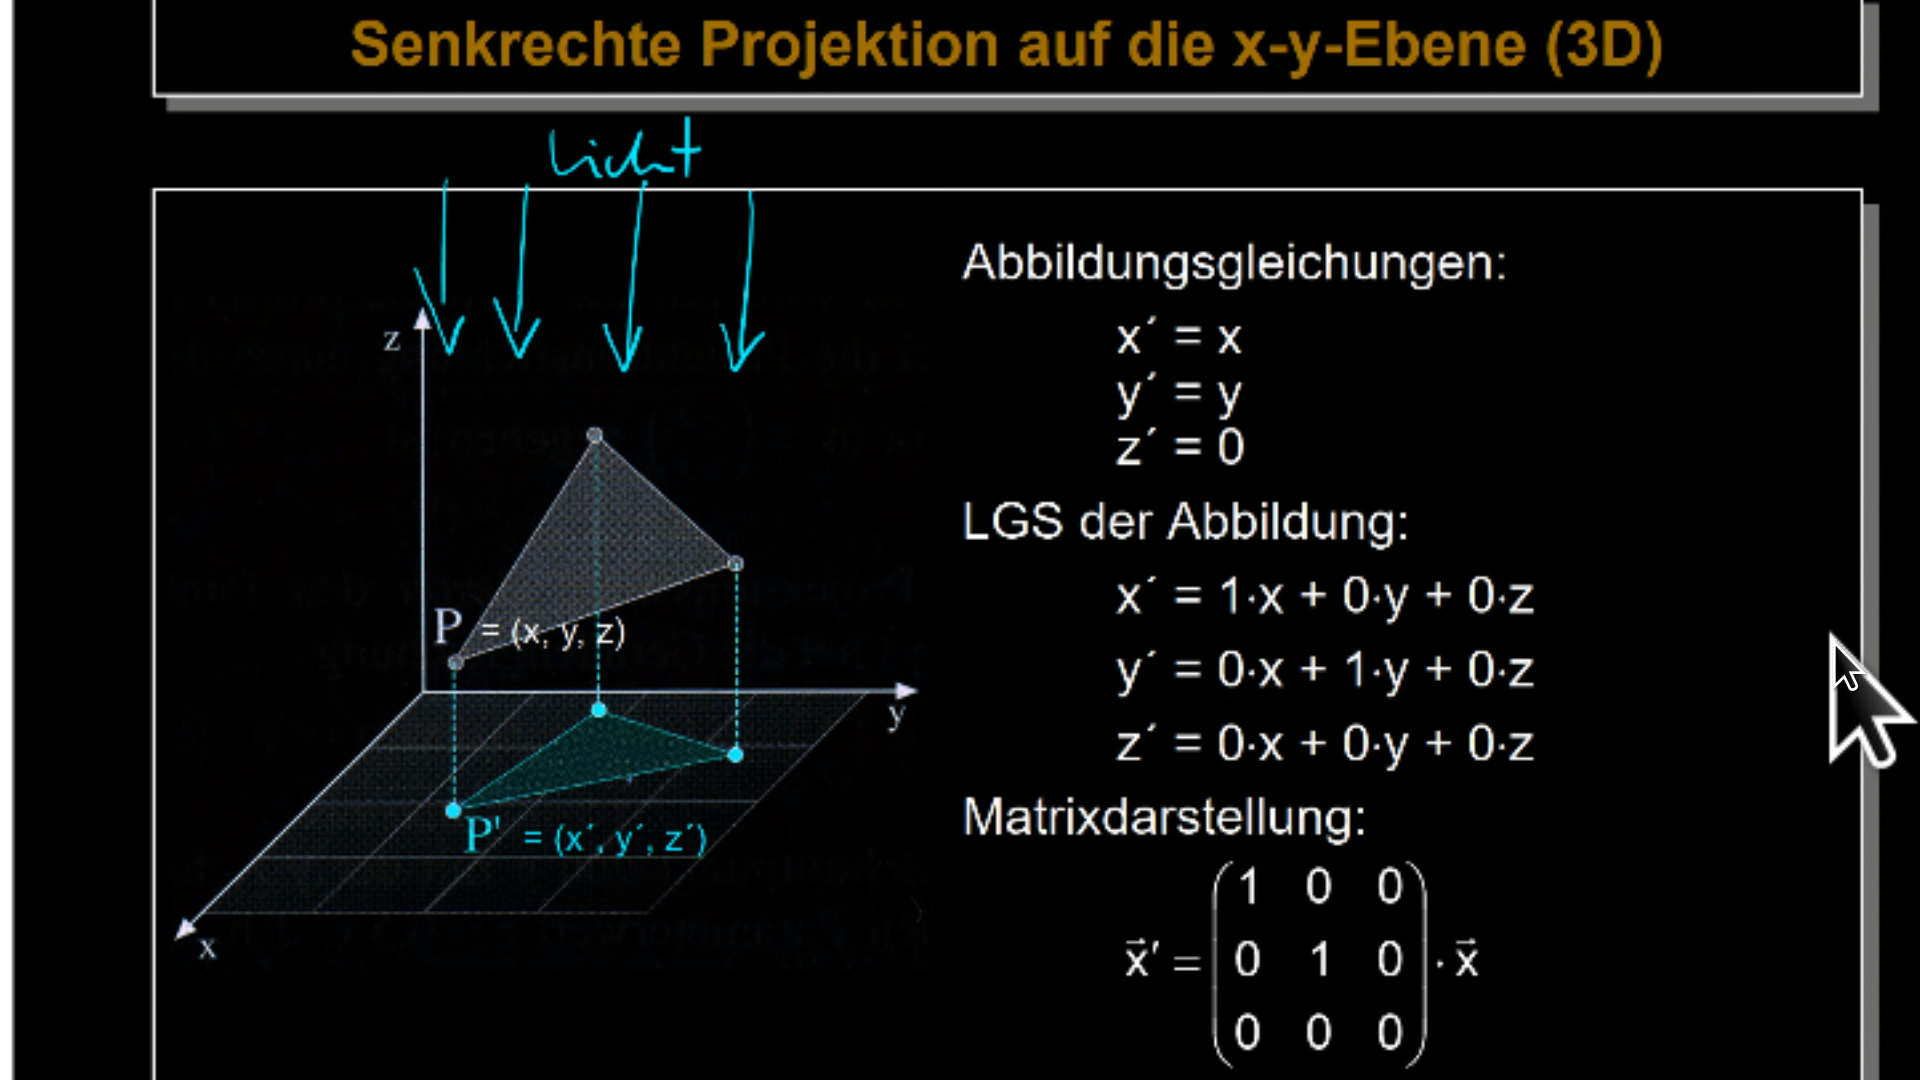
\includegraphics[width=\linewidth]{proschatten}
	Ansatz wie oben. Unterschied: Ebene in die gespiegelt wird behält ihre Koordinaten. Rest = 0 \\
	Def. Eine Funktion f: $R^n \to R^m$ die jedem Punkt mit dem Ortsvektor $\vec{x}$ genau einen Punkt mit dem Ortsvektor $\vec{x'}$ zuordnet, heißt lineare Abbildung, wenn es eine mxn Matrix A gibt  mit: $\vec{x'}$ = A $\cdot$ $\vec{x}$ Dann heißt A Abbildungsmatrix  von f. \\
	Satz: die Spalten der Abbildungsmatrix sind die Bilder der Einheitsvektoren!!! \\
	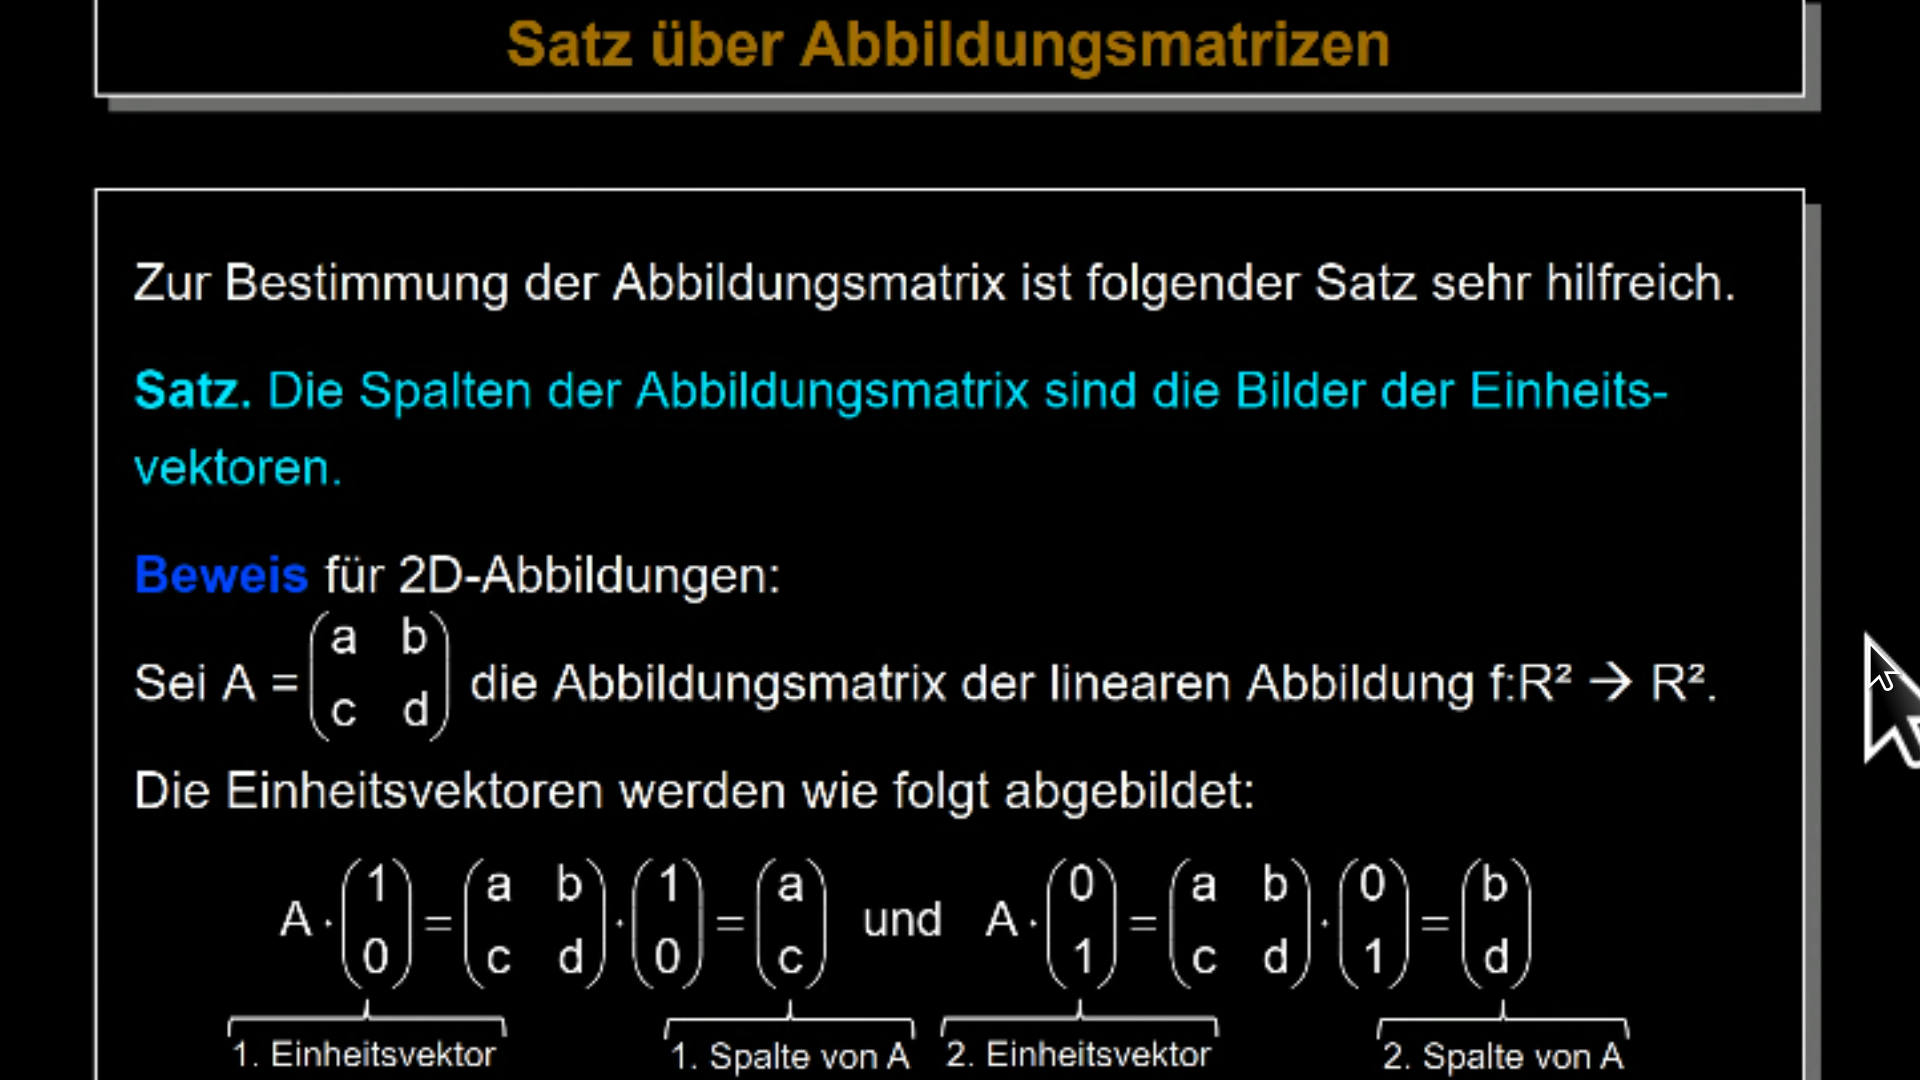
\includegraphics[width=\linewidth]{satz} \\
	Übung für obigen Satz \\
	\includegraphics[width=\linewidth]{üsatz}
	\subsection*{08.09.2021}
	Die Bilder der Einheitsvektoren sind die Spalten der Abbildungsmatrix. \\
	Drehung gilt auch für obigen Satz. \\
	$\left(\begin{array}{cc}
	cos(\phi) & -sin(\phi) \\ sin(\phi) & cos(\phi)
	\end{array}\right)$ \\
	Sofern nicht anders vereinbart: Drehung GEGEN den Uhrzeigersinn. \\
	Mehrere Projektionen: Matrizen nacheinander multiplizieren. \\
	Multiplikation von links. \\
	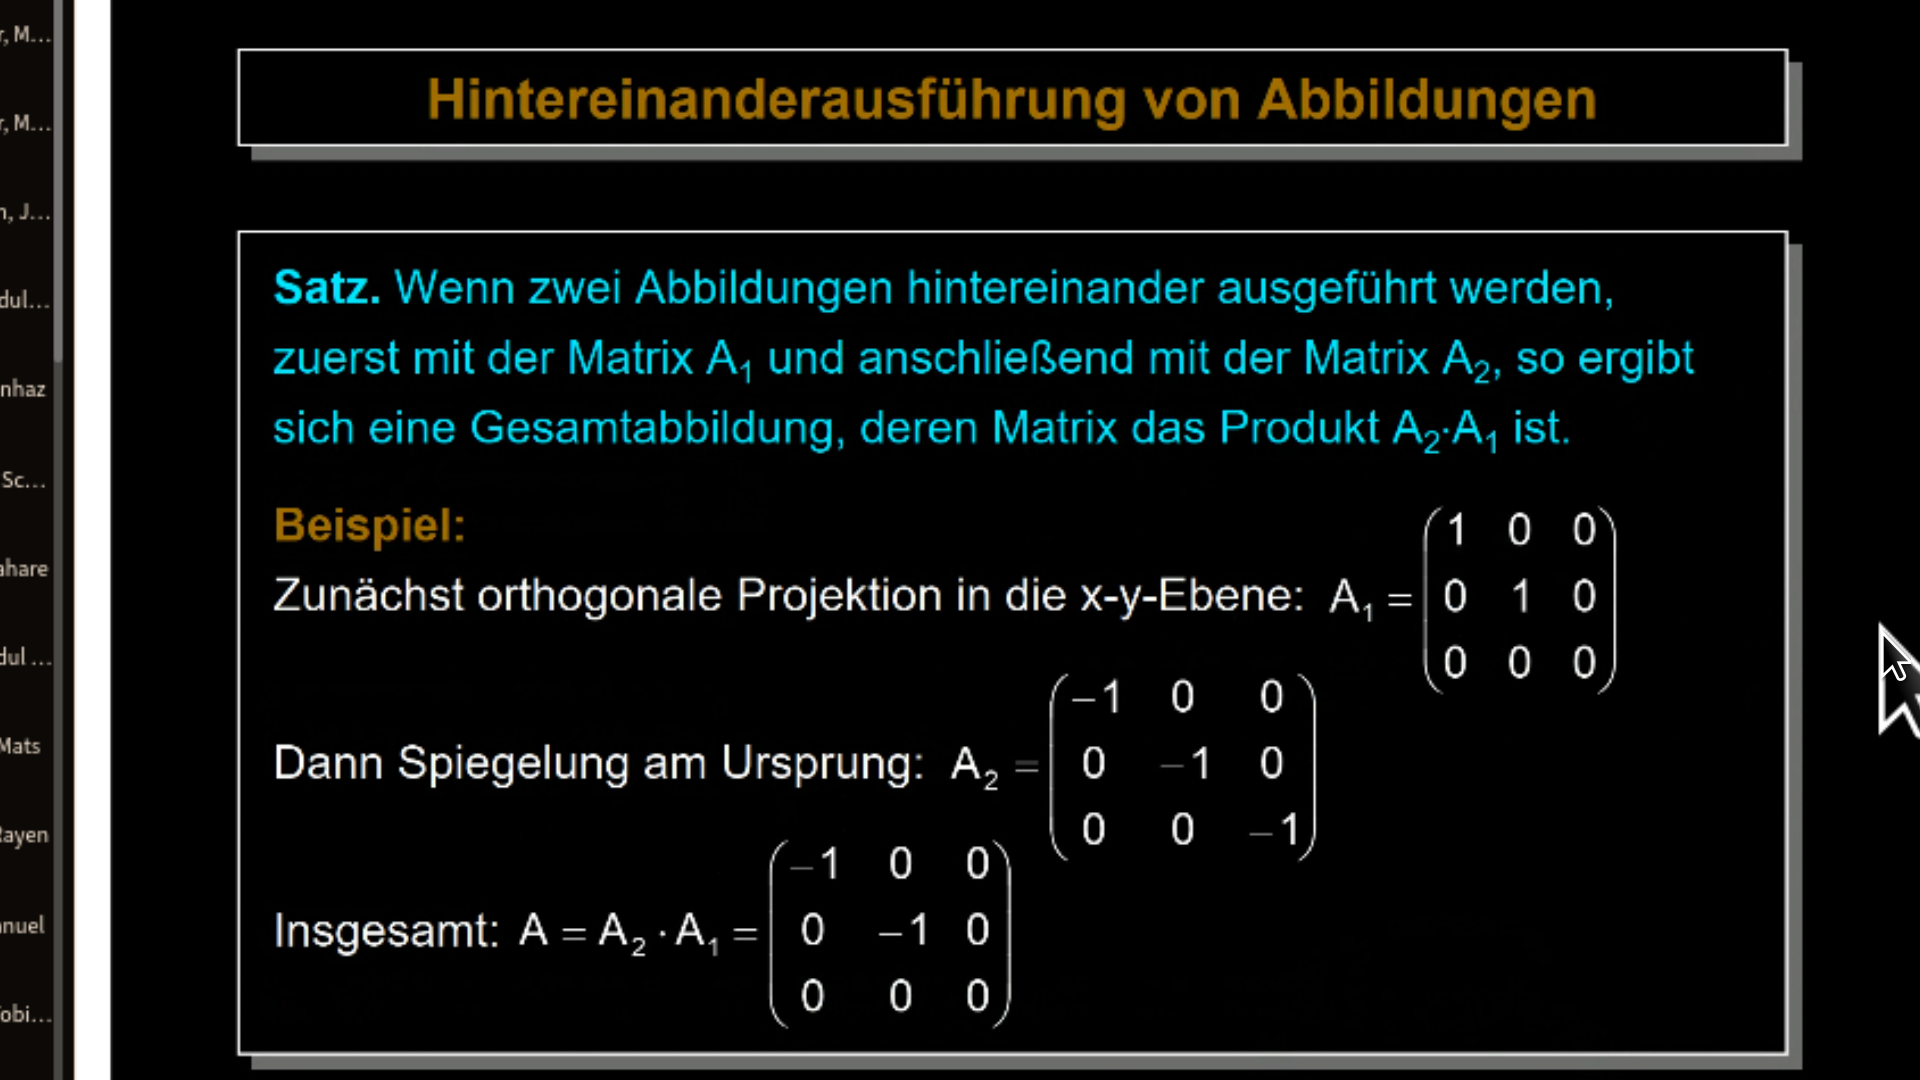
\includegraphics[width=\linewidth]{abbildung} \\
	Kern einer Abbildung \\
	Bild einer Abbildung \\
	Bild ist die Menge aller Bildpunkte. \\
	Kern besteht mindestens aus 0 Punkt \\
	Vektoren, die auf sich selbst abbilden nennt man Fixpunkte. \\
	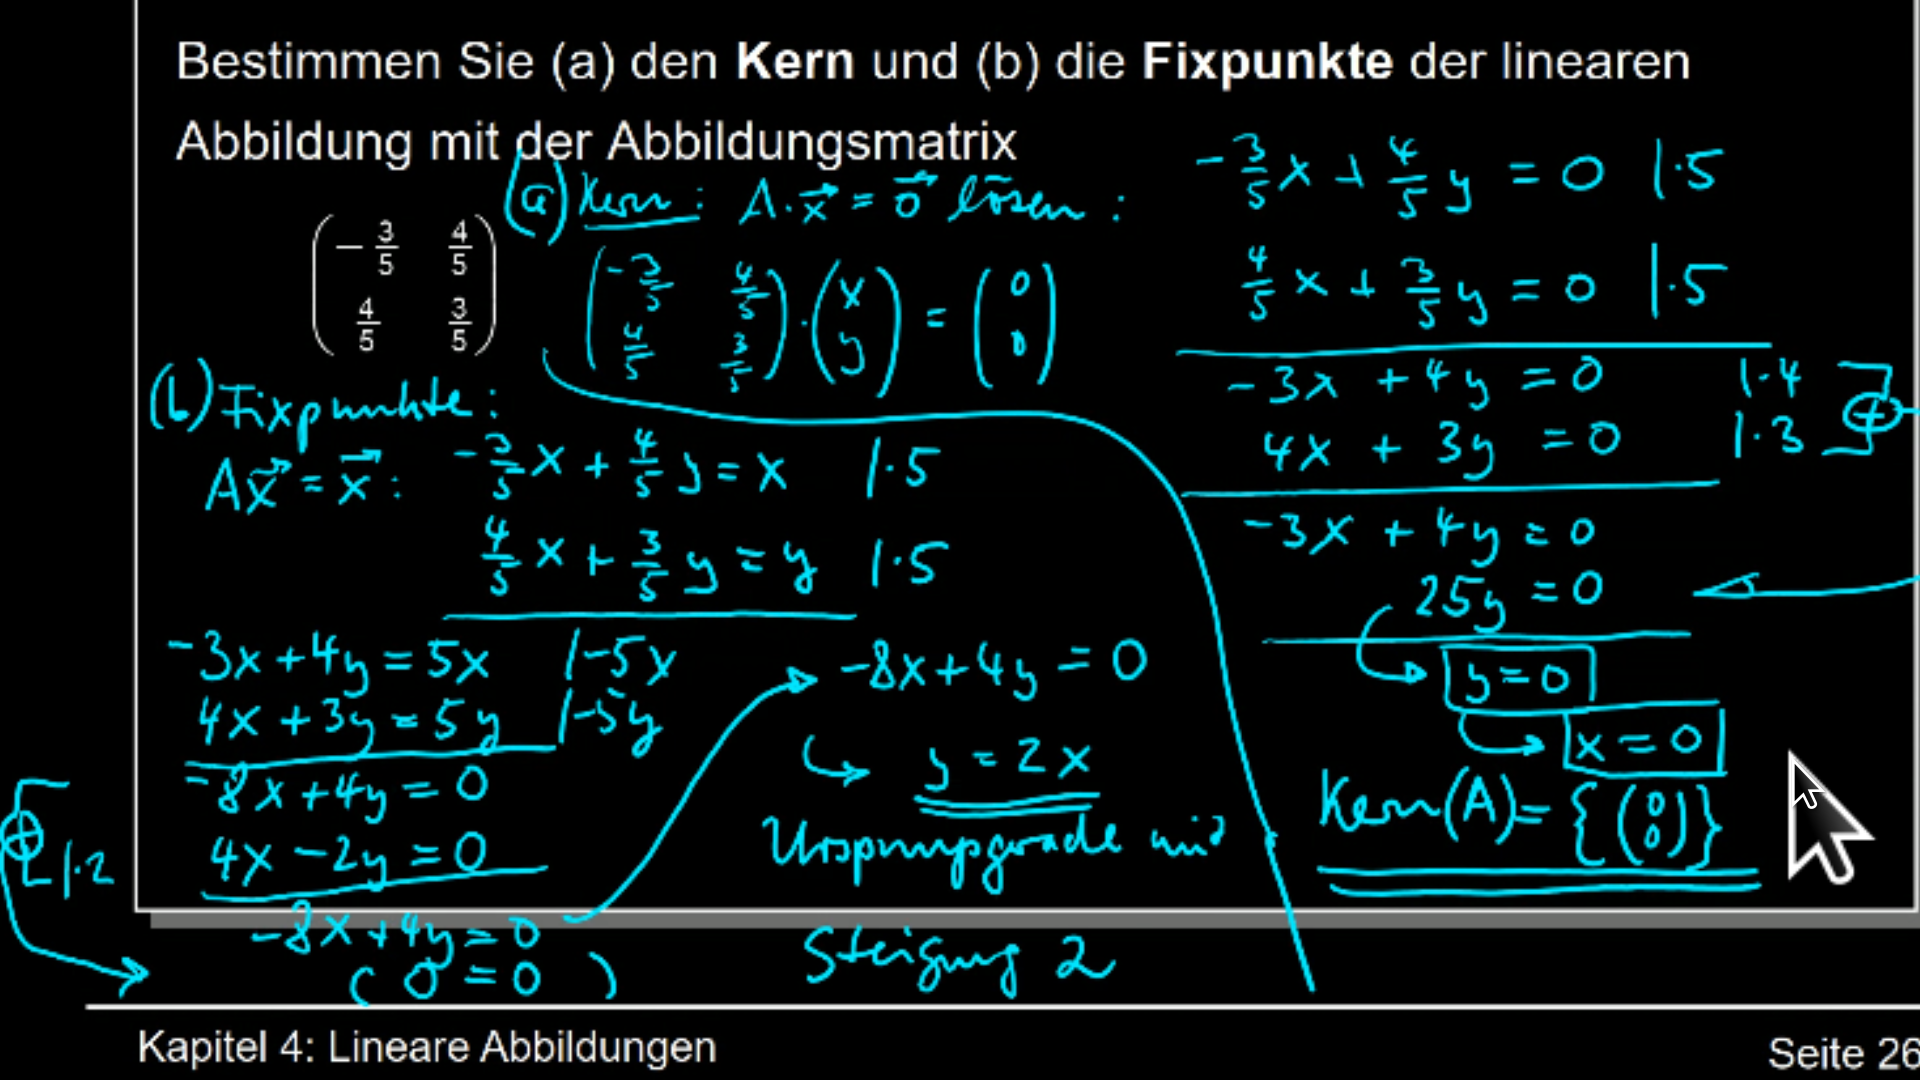
\includegraphics[width=\linewidth]{sampleFixKern}
	\subsection*{14.06.2021}
	Koordinatensysteme anpassen \\
	Eigenvektor ungleich Nullvektor sodass Vektor in die gleiche Richtung zeigt aber gestreckt oder gestaucht ist. \\
	Eigenwerte berechnen mit charateristischem Polynom \\
	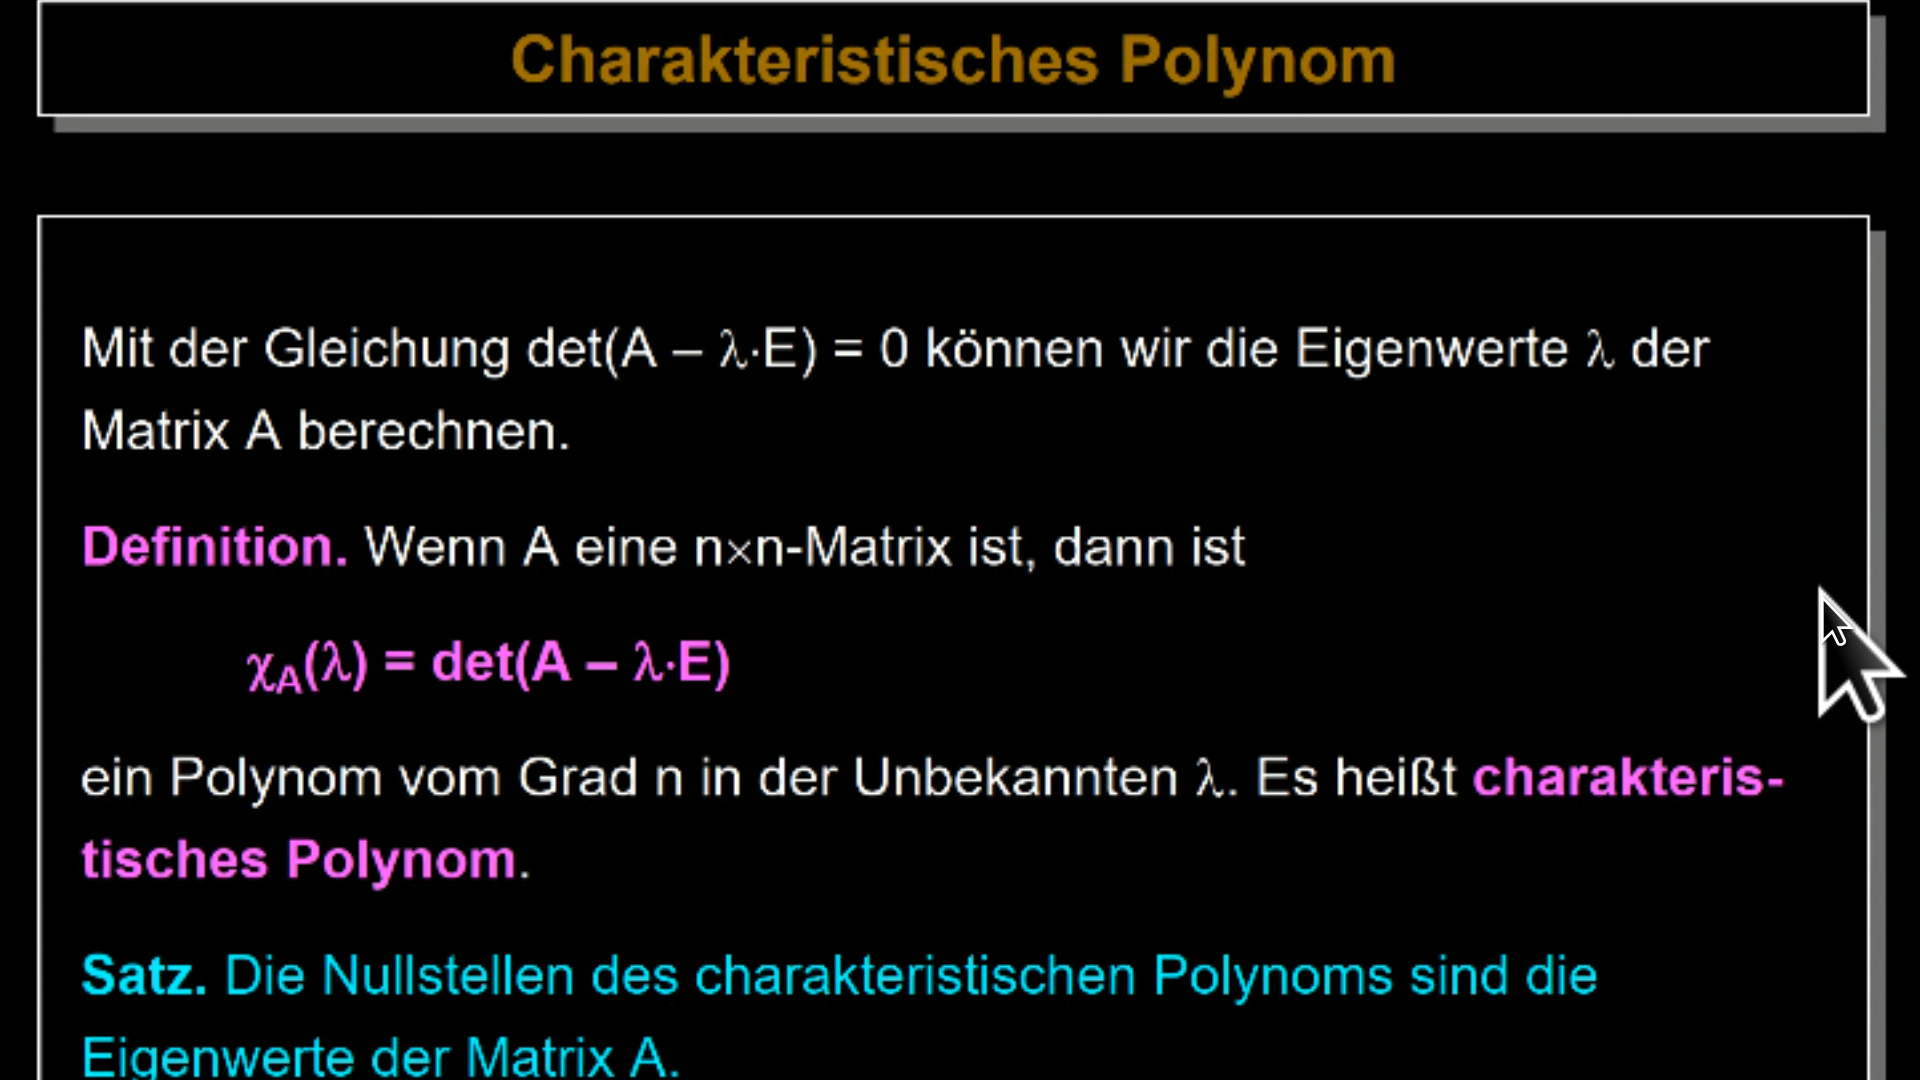
\includegraphics[width=\linewidth]{charpolynom} \\
	Eigenwert Problem bei Quantencomputing \\
	Eigenwert bestimmen dann Eigenvektor bestimmen. \\
	Basis: Menge aus n linear unabhängigen Vektoren im n-dimensionalen Raum. \\
	Koordinaten sind Linearkombinationen der Basis. \\
	Koordinatentransforamtion: Die Vektoren der Basis sind Spalten der Transformationsmatrix \\
	Stichwort Basistransformation. \\
	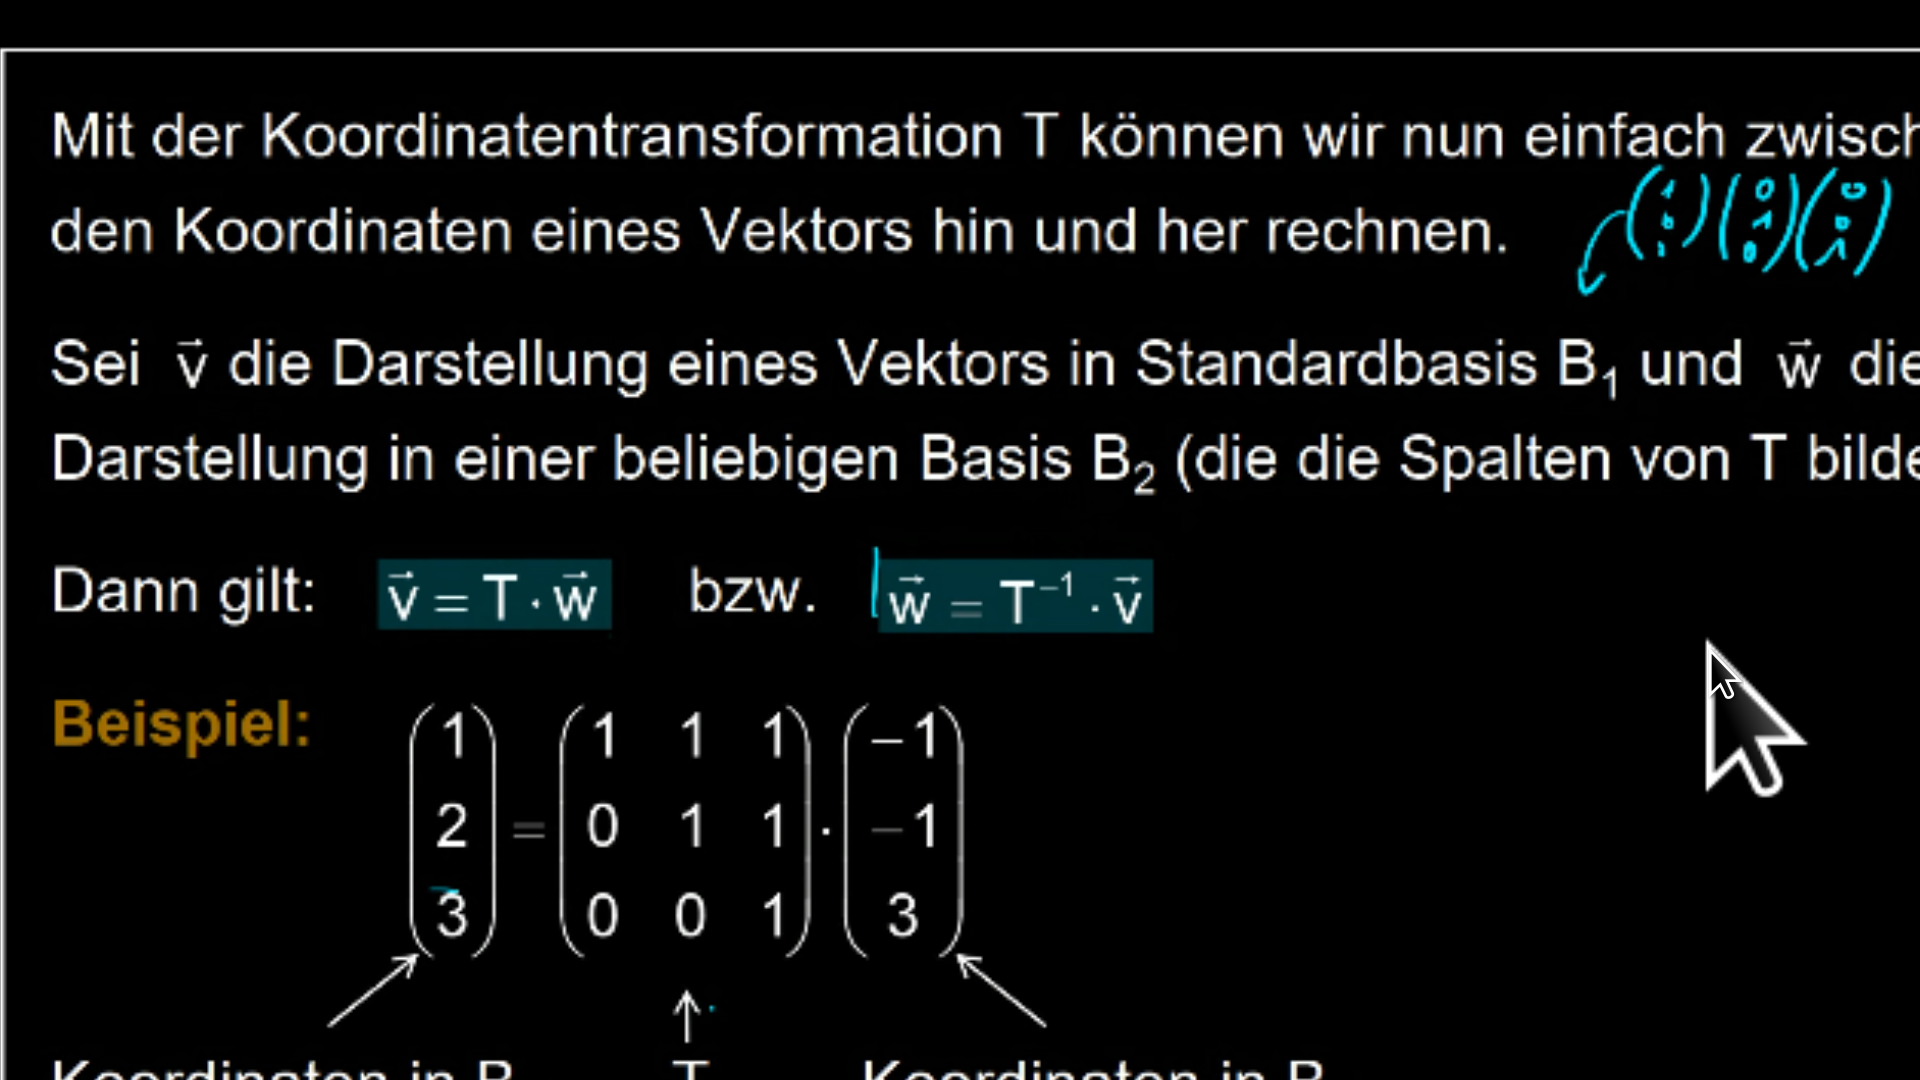
\includegraphics[width=\linewidth]{transformer} 
	\subsection*{22.06.21}
	$B = T^-1 \cdot A \cdot T$ \\
	Schreibe T als Matrix mit den Vektoren der neuen Basis als Spalten. \\
	Einfach, wenn Matriax in Diagonalform. \\
	Suche Basis in der  A Diagonalform hat \\
	wenn möglich heist A diagonalisierbar. \\
	Tipp: Eigenvektoren als Spalten für B verwenden. \\
	multipliziere von rechts nach links !!!
	Wenn es n verschiedene Eigenwerte gibt, ok cool \\
	ansonsten zweites Kriterium: Genau dann wenn zwei Bedingungen 1. char. Polynom muss zerfallen in lineare Faktoren. Vielfaches von Eigenwerta \\
	2. Anzahl der linear unabhängigen Eigenvektoren muss dem Vielfaches des Vektors entsprechen.
	Algebraische Strukturen \\
	Körper, komplexe Zahlen, Vektorraum \\
	Vektorraumbegriff verallgemeinert \\
	Körper sind Strukturen mit Gesetzen \\
	Innerhalb des Köpers kann wie mit reellen Zahlen gerechnet werden \\
	Dafür muss gelten: Neutrales Element Assoziativität und Kommutativität für + und $\cdot$ \\
	neutrales Element bzgl + und $\cdot$ \\
	Distributivgesetz gilt \\
	Körper kann $\infty$ Elemente oder endlich viele Elemente enthalten \\
	Q ist z.B. unendlich \\
	Es gibt Körper mit Primzahlpotenz als Anzahl der Elemente. \\
	Primzahlpotenz \\
	komplexe Zahlen \\
	i \\
	Komplexe Zahl (a, b) Realteil und Imaginärteil \\
	komplexe Zahlen lassen sich als Vektoren darstellen \\
	imaginäre Einheit \\
	i * i = -1 \\
	z = a + i * b \\
	Summendarstellung
	\subsection*{29.06.2021}
	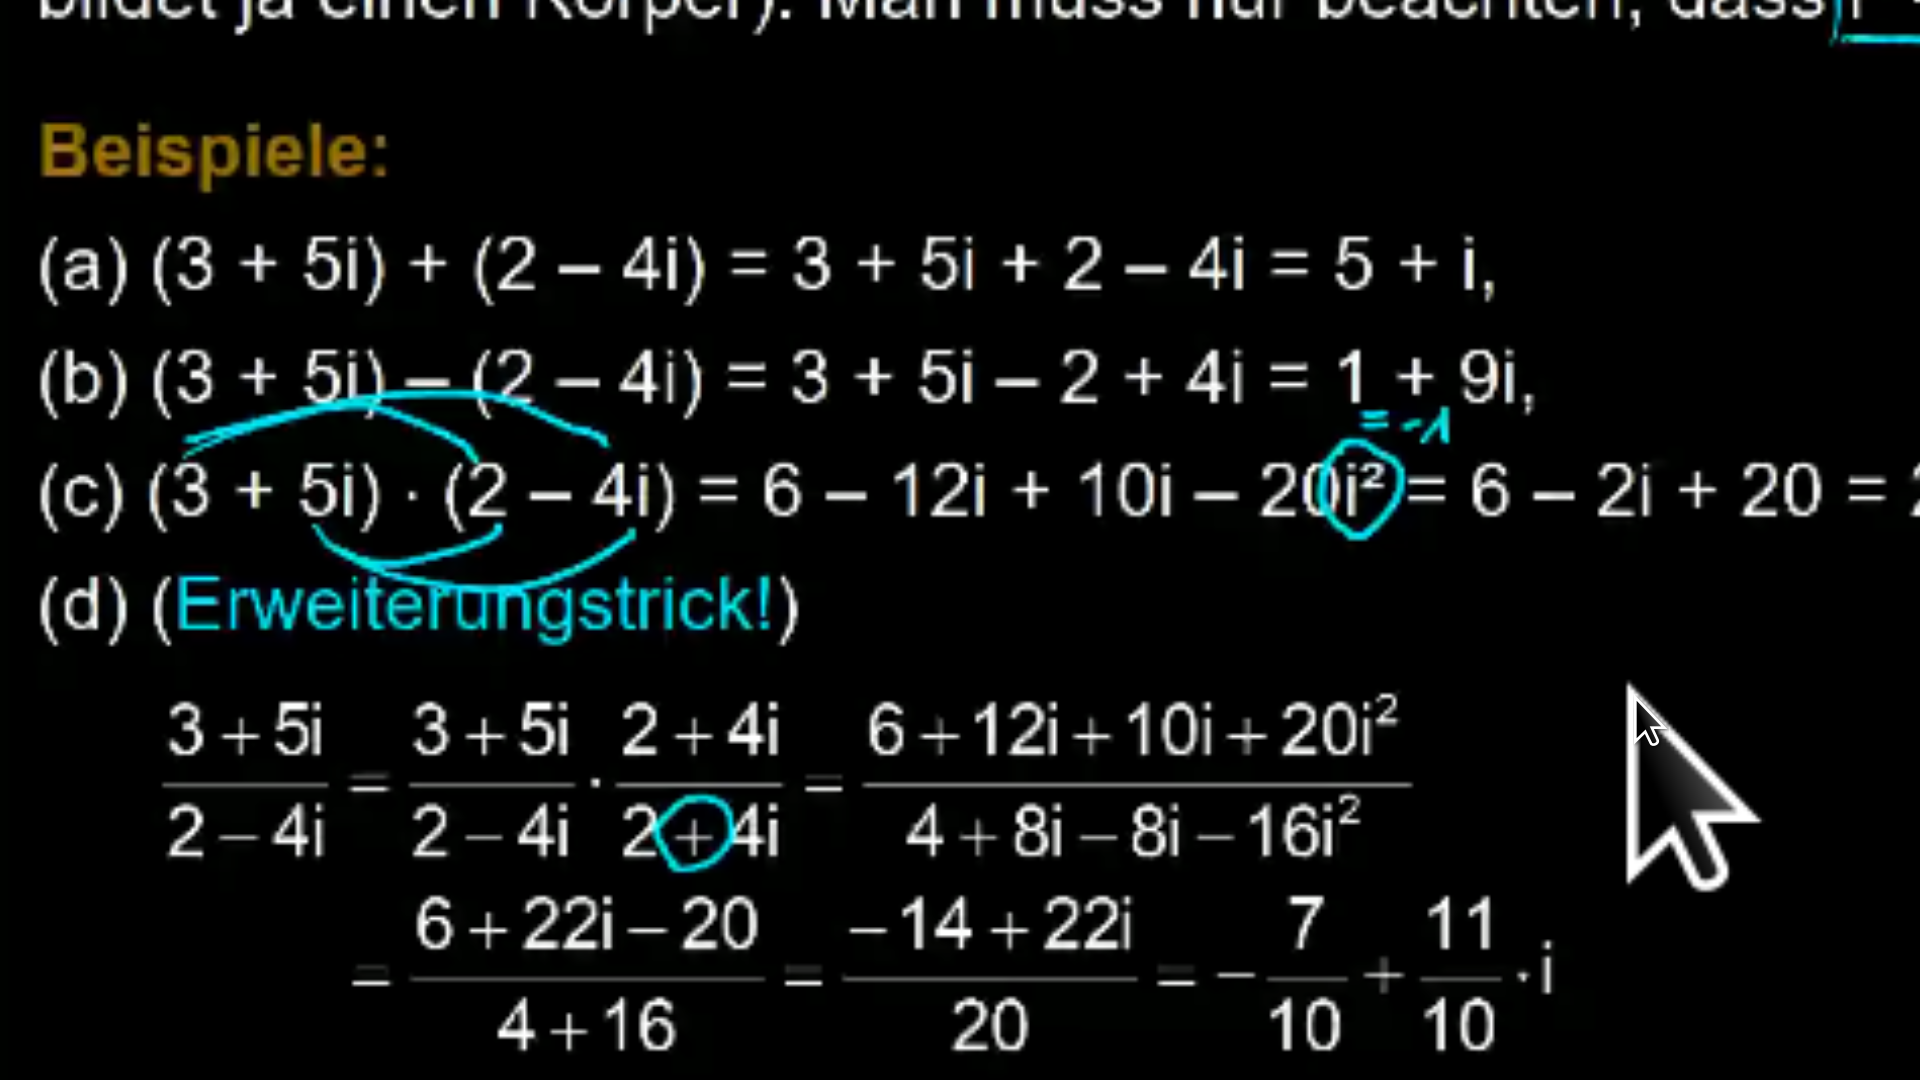
\includegraphics[width=\linewidth]{samplekz} \\ \\
	Vergleiche Betrag bei imaginären Zahlen \\
	Betrag ist Abstand vom Ursprung \\
	trigonometrische Darstellung \\
	z = $\phi$ * r \\
	denke an Pythagoras \\
	Annäherung mit Taylorpolynom \\
	$x^{n}$ hat in C n Lösungen \\
	\subsection*{06.07.2021}
	Vektorräume \\
	Zusammenfassung strukturgleicher Objekte \\
	Vektorraum über Objekt K mit V Elementen V sind Vektoren \\
	Vervielfachung \\
	Rechnen wie in $R^{n}$ \\
	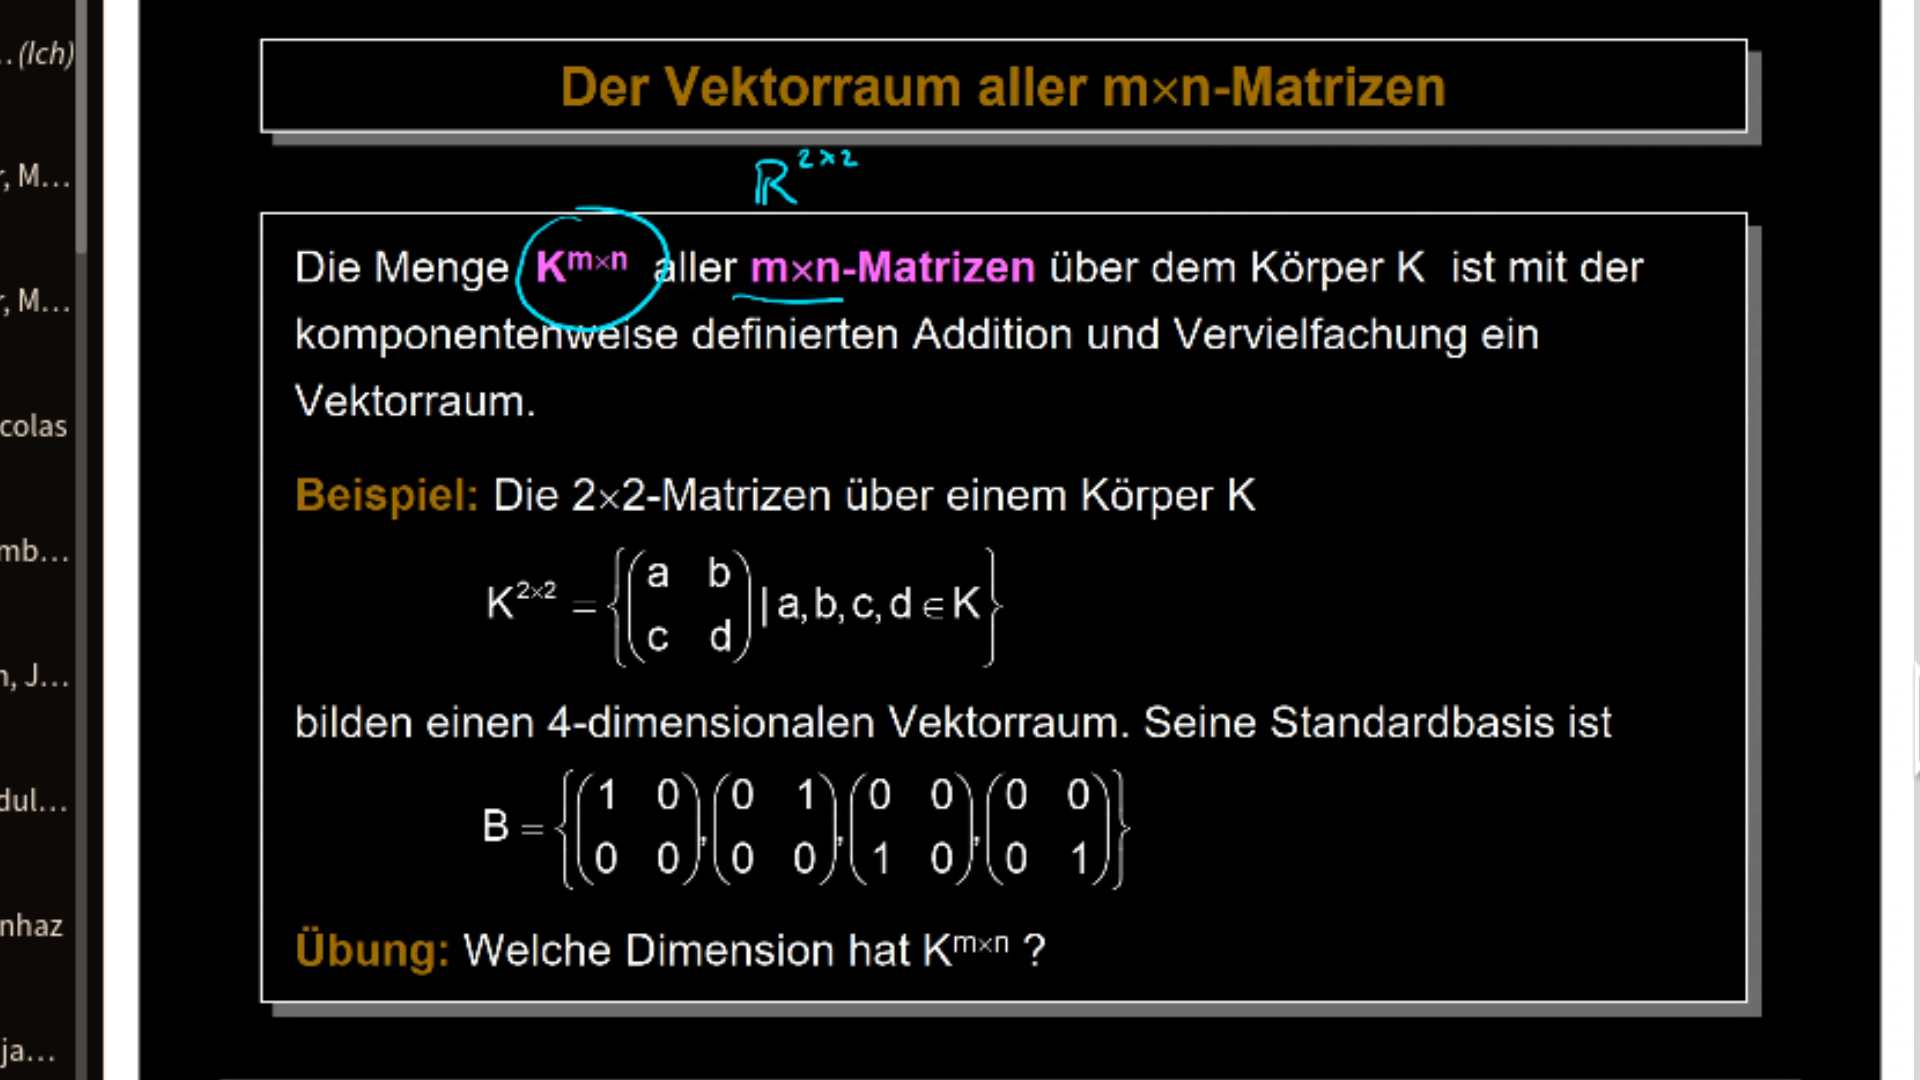
\includegraphics[width=\linewidth]{mav} \\
	Vektorraum $K^{mxn}$  hat die Dimension m $\cdot$ n \\
	Matrizen einer festen Ordnung bilden einen Vektorraum. \\
	Dimension ist die Anzahl der Elemente der Basis \\
	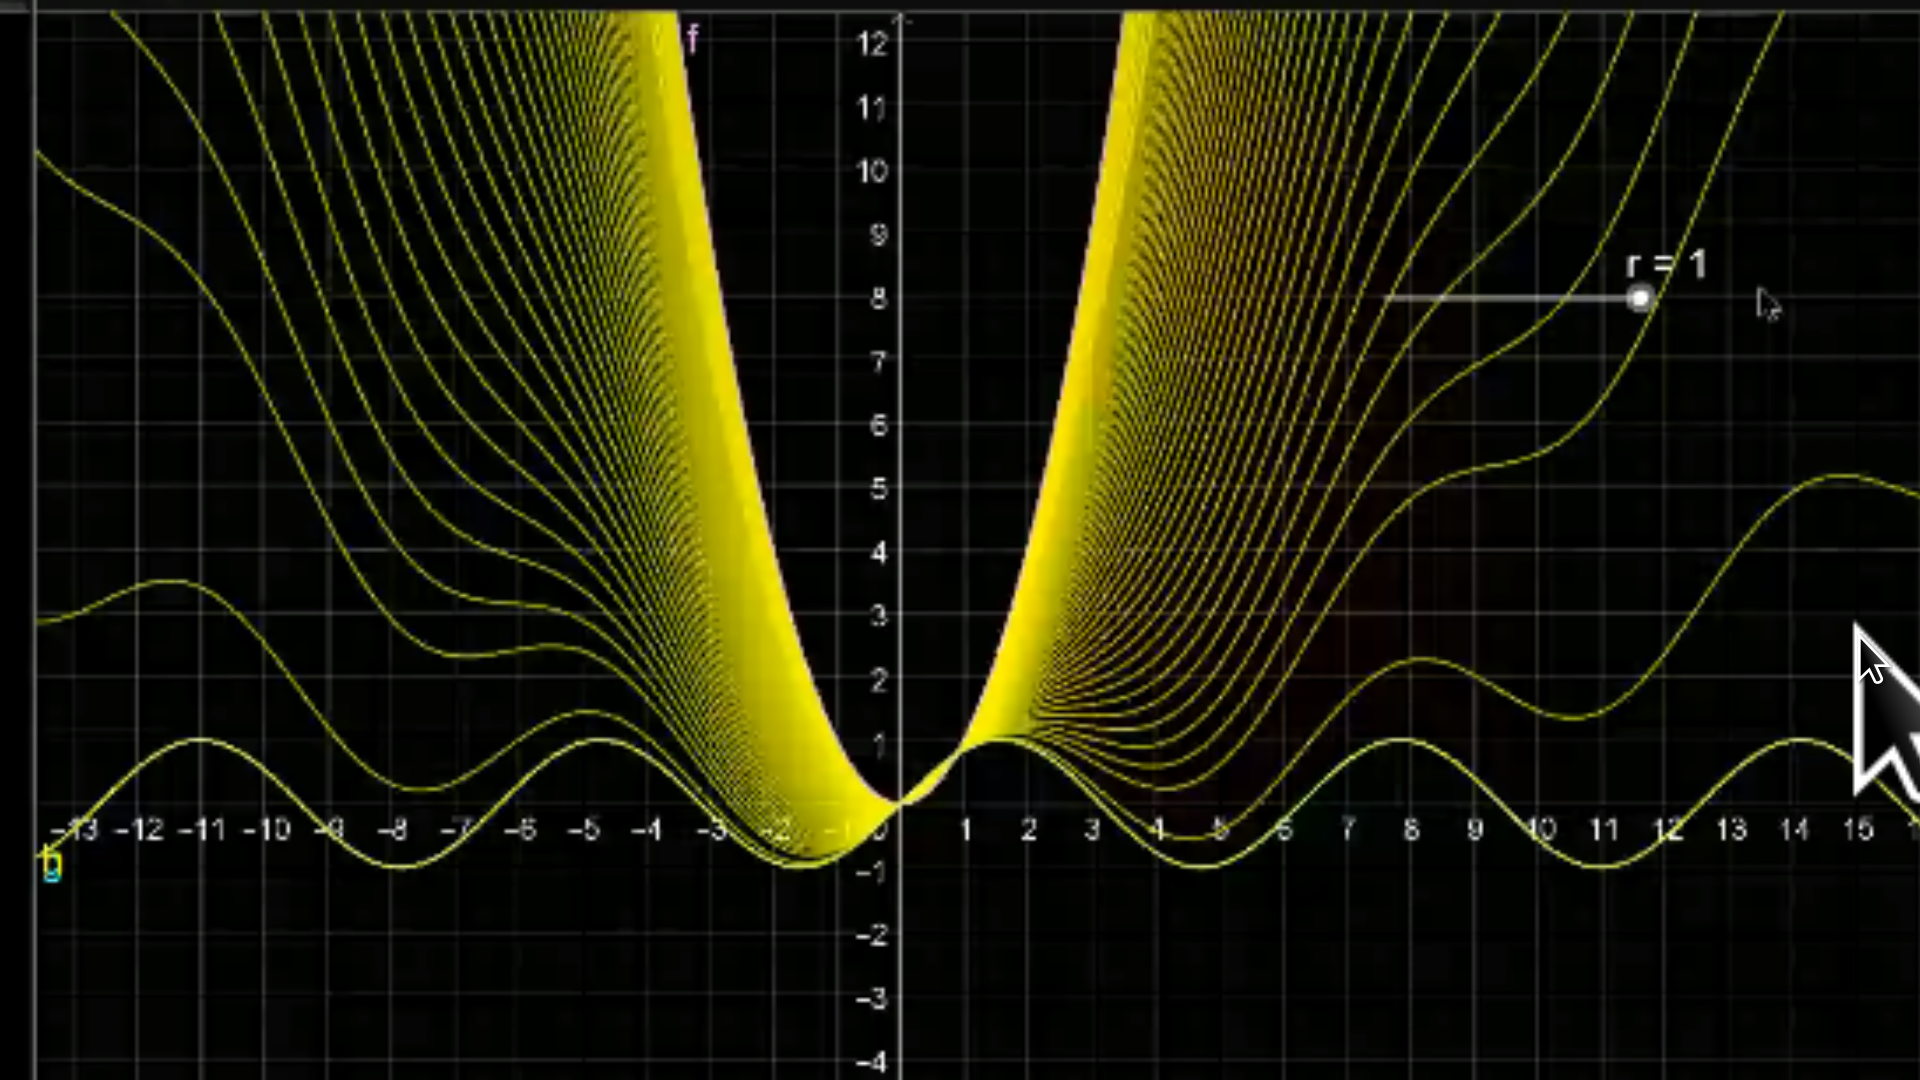
\includegraphics[width=\linewidth]{streckeinv} \\
	Strecke zwischen zwei Funktionen im Vektorraum. \\
	Morphing \\

\end{document}